% VLDB-Template enhances the ACM master template, acmart.cls v2.19 (2026/06/27):
% https://www.acm.org/publications/proceedings-template
% The ACM Latex guide provides further information about the ACM template
%
% This bundle pins acmart.cls v2.19 (rather than relying on whatever version
% ships with an author's local TeX install or Overleaf project) to guarantee
% consistent formatting across all PVLDB submissions.

\documentclass[sigconf, nonacm]{acmart}

%%% do not modify the following VLDB block %%
%%% VLDB block start %%%
\usepackage{pvldb}% VLDB/PVLDB formatting overrides, see pvldb.sty for details.
                      % Do not remove -- required for consistent proceedings
                      % formatting across all VLDB submissions.
%%% VLDB block end %%%

\usepackage{algorithmic}
\usepackage{graphicx}
\usepackage{textcomp}
\usepackage{xcolor}
\usepackage{hyperref}
\usepackage{wrapfig}
\usepackage[many]{tcolorbox}    	% for COLORED BOXES (tikz and xcolor included)
\usepackage{setspace}               % for LINE SPACING
\usepackage{multicol}
\usepackage{caption}
\usepackage[ruled,vlined]{algorithm2e}

%% The following must be set for each paper (values below are placeholders).
%% Everything else (volume/issue/year defaults, the PVLDB Reference Format
%% block, license footer, and Artifact Availability block) is handled by
%% pvldb.sty -- see that file if you need to change shared defaults.
\renewcommand\vldbdoi{XX.XX/XXX.XX}
\renewcommand\vldbpages{XXX-XXX}
% leave empty if no availability url should be set
\renewcommand\vldbavailabilityurl{URL_TO_YOUR_ARTIFACTS} 

\begin{document}
\title{ASZ: Hierarchical Configuration Tuning for Prediction-Based Error-Bounded Lossy Compression}

%%
%% The "author" command and its associated commands are used to define the authors and their affiliations.
%1
\author{Zizhe Jian}
\affiliation{%
  \institution{University of California, Riverside}
  \city{Riverside}
  \state{California}
  \country{United States}
}
\email{zjian106@ucr.edu}
%2
\author{Yafan Huang}
\affiliation{%
  \institution{University of Maryland, College Park}
  \city{College Park}
  \state{Maryland}
  \country{United States}
}
\email{yafan@umd.edu}
%3
\author{Zhuoxun Yang}
\affiliation{%
  \institution{Florida State University}
  \city{Tallahassee}
  \state{Florida}
  \country{United States}
}
\email{zy24b@fsu.edu}
%4
\author{Sheng Di}
\affiliation{%
  \institution{Argonne National Laboratory}
  \city{Lemont}
  \state{Illinois}
  \country{United States}
}
\email{sdi1@anl.gov}
%5
\author{Bo Jiang}
\affiliation{%
  \institution{Temple University}
  \city{Philadelphia}
  \state{Pennsylvania}
  \country{United States}
}
\email{jiang.bo@temple.edu}
%6
\author{Shixun Wu}
\affiliation{%
  \institution{University of California, Riverside}
  \city{Riverside}
  \state{California}
  \country{United States}
}
\email{swu264@ucr.edu}
%7
\author{Jiajun Huang}
\affiliation{%
  \institution{University of South Florida}
  \city{Tampa}
  \state{Florida}
  \country{United States}
}
\email{jiajunhuang@usf.edu}
%8
\author{Kai Zhao}
\affiliation{%
  \institution{University of California, Riverside}
  \city{Riverside}
  \state{California}
  \country{United States}
}
\email{kai.zhao@fsu.edu}
%10
\author{Jinyang Liu}
\affiliation{%
  \institution{Shanghai Jiao Tong University}
  \city{Shanghai}
  \country{China}
}
\email{jinyang.liu@sjtu.edu.cn}
%11
\author{Robert Underwood}
\affiliation{%
  \institution{Argonne National Laboratory}
  \city{Lemont}
  \state{Illinois}
  \country{United States}
}
\email{runderwood@anl.gov}
%12
\author{Miaoqi Chu}
\affiliation{%
  \institution{Argonne National Laboratory}
  \city{Lemont}
  \state{Illinois}
  \country{United States}
}
\email{mqichu@anl.gov}
%13
\author{Peco Myint}
\affiliation{%
  \institution{Argonne National Laboratory}
  \city{Lemont}
  \state{Illinois}
  \country{United States}
}
\email{pmyint@anl.gov}
%14
\author{Nicholas Schwarz}
\affiliation{%
  \institution{Argonne National Laboratory}
  \city{Lemont}
  \state{Illinois}
  \country{United States}
}
\email{nschwarz@anl.gov}
%15
\author{Sian Jin}
\affiliation{%
  \institution{Temple University}
  \city{Philadelphia}
  \state{Pennsylvania}
  \country{United States}
}
\email{sian.jin@temple.edu}
%16
\author{Zizhong Chen}
\affiliation{%
  \institution{University of California, Riverside}
  \city{Riverside}
  \state{California}
  \country{United States}
}
\email{chen@cs.ucr.edu}
%17
\author{Franck Cappello}
\affiliation{%
  \institution{Argonne National Laboratory}
  \city{Lemont}
  \state{Illinois}
  \country{United States}
}
\email{cappello@mcs.anl.gov}

%%
%% The abstract is a short summary of the work to be presented in the
%% article.
% 科学数据系统需要针对 data characteristics 和 quality targets 自动选择 compression configurations；
% configuration evaluation 需要完整 compression，导致只能搜索很小空间；
% ASZ 将 configuration evaluation 分解成 RD-aware objective、entropy-distortion proxy、reusable residual statistics；
% 在 interpolation compressor 中实例化为 joint stencil/coefficient search；
% 搜索规模、估计 speedup、oracle regret；
% 最终 RD gain、runtime、跨 timestep amortization；
% 非预测 compressor 上的 selector generality。

\begin{abstract}
Error-bounded lossy compression is widely used to reduce storage, I/O, and data-movement costs in scientific data management. The performance of a lossy compressor, however, depends not only on its underlying compression algorithm but also on how its configurable components are selected and organized for the target data. Existing compressors typically explore only limited configuration spaces or evaluate candidate configurations by repeatedly executing expensive compression pipelines, making systematic tuning difficult.

In this paper, we propose a hierarchical configuration-tuning framework that organizes tuning decisions according to their potential benefit, evaluation cost, and scope of reuse. We use this framework to systematically analyze the tunable dimensions of prediction-based error-bounded compressors, including stencil patterns, predictor coefficients, and traversal orders, among others. We also develop accurate and inexpensive proxy metrics that enable efficient evaluation of candidate configurations. Based on these findings, we develop ASZ, which applies the resulting tuning strategies at their appropriate stages.

Experiments on eight datasets from different domains show that ASZ consistently improves rate–distortion performance over state-of-the-art prediction-based compressors while maintaining comparable compression time. Compared with QoZ, ASZ commonly achieves up to 2× higher compression ratios at the same reconstruction quality, with improvements exceeding 10× on highly anisotropic datasets. These results demonstrate that hierarchical configuration tuning is an effective and practical approach for improving error-bounded lossy compression.
\end{abstract}

\maketitle

%%% do not modify the following VLDB block %%
%%% VLDB block start %%%
\vldbtopmatter
%%% VLDB block end %%%

\definecolor{main}{HTML}{464646}    % setting main color to be used
\definecolor{sub}{HTML}{efefef}     % setting sub color to be used

\tcbset{
    sharp corners,
    colback = white,
    before skip = 0.2cm,    % add extra space before the box
    after skip = 0.5cm      % add extra space after the box
}                           % setting global options for tcolorbox

% You can copy any following box you like to your code.
\newtcolorbox{boxA}{
    fontupper = \bf,
    boxrule = 1.5pt,
    colframe = black % frame color
}

\newtcolorbox{boxB}{
    fontupper = \bf\color{main}, % font color
    boxrule = 1.5pt,
    colframe = main,
    rounded corners,
    arc = 5pt   % corners roundness
}

\newtcolorbox{boxC}{
    colback = sub, % background color
    boxrule = 0pt  % no borders
}

\newtcolorbox{boxD}{
    colback = sub, 
    colframe = main, 
    boxrule = 0pt, 
    toprule = 3pt, % top rule weight
    bottomrule = 3pt % bottom rule weight
}

\newtcolorbox{boxE}{
    enhanced, % for a fancier setting,
    boxrule = 0pt, % clearing the default rule
    borderline = {0.75pt}{0pt}{main}, % outer line
    borderline = {0.75pt}{2pt}{sub} % inner line
}

\newtcolorbox{boxF}{
    colback = sub,
    enhanced,
    boxrule = 1.5pt, 
    colframe = white, % making the base for dash line
    borderline = {1.5pt}{0pt}{main, dashed} % add "dashed" for dashed line
}

\newtcolorbox{boxG}{
    enhanced,
    boxrule = 0pt,
    colback = sub,
    borderline west = {1pt}{0pt}{main}, 
    borderline west = {0.75pt}{2pt}{main}, 
    borderline east = {1pt}{0pt}{main}, 
    borderline east = {0.75pt}{2pt}{main}
}

\newtcolorbox{boxH}{
    colback = sub, 
    colframe = main, 
    boxrule = 0pt, 
    leftrule = 6pt % left rule weight
}

\newtcolorbox{boxI}{
    colback = sub, 
    colframe = main, 
    boxrule = 0pt, 
    toprule = 6pt % top rule weight
}

\newtcolorbox{boxJ}{
    sharpish corners, % better drop shadow
    colback = sub, 
    colframe = main, 
    boxrule = 0pt, 
    toprule = 4.5pt, % top rule weight
    enhanced,
    fuzzy shadow = {0pt}{-2pt}{-0.5pt}{0.5pt}{black!35} % {xshift}{yshift}{offset}{step}{options} 
}

\newtcolorbox{boxK}{
    sharpish corners, % better drop shadow
    boxrule = 0pt,
    toprule = 4.5pt, % top rule weight
    enhanced,
    fuzzy shadow = {0pt}{-2pt}{-0.5pt}{0.5pt}{black!35} % {xshift}{yshift}{offset}{step}{options} 
}

\newtcolorbox{boxL}{
    fontupper = \color{main},
    rounded corners,
    arc = 6pt,
    colback = sub, 
    colframe = main!50, 
    boxrule = 0pt, 
    bottomrule = 4.5pt 
}

\newtcolorbox{boxM}{
    fontupper = \color{white},
    rounded corners,
    arc = 6pt,
    colback = main!80, 
    colframe = main, 
    boxrule = 0pt, 
    bottomrule = 4.5pt,
    enhanced,
    fuzzy shadow = {0pt}{-3pt}{-0.5pt}{0.5pt}{black!35}
}
\section{Introduction}

% prediction-based compression重要
The volume of scientific data generated by high-performance computing (HPC) simulations and scientific instruments continues to grow rapidly, placing increasing pressure on storage systems, I/O bandwidth, and data movement~\cite{lockwood2017storage,huang2023towards,lewis2025machine,giannakou2024understanding,lockwood2019understanding}. Error-bounded lossy compression has emerged as an important technique for alleviating these challenges~\cite{cappello2019use,di2025survey,cappello2025support}, as it substantially reduces data volume while preserving user-specified accuracy~\cite{lindstrom2014fixed,di2016fast,huang2023cuszp,gong2023mgard,li2023lossy}.

% 现有方法中的tuning
Achieving strong compression performance requires more than finding better compression algorithm. It also depends critically on how the compressor is configured for the target data and the user’s compression objective. These configurations may include not only parameter values, but also which compression components are executed and how they are organized. Consequently, different configurations of the same compressor can exhibit substantially different compression ratios and data distortion. For example, QoZ~\cite{liu2022dynamic,liu2024high}, a prediction-based compressor, dynamically selects among candidate predictors during online compression according to the input data. At the compressor-design level, transform-based compressors such as ZFP~\cite{lindstrom2014fixed,diffenderfer2019error} have continued to evolve through refinements to their transform designs and coding strategies. At an even coarser level, some compression frameworks~\cite{liang2019significantly} combine multiple existing compressors and select which compressor to invoke for a particular dataset or data field.

% 现有方法中tuning的问题
Despite the strong performance achieved by existing compressors and tuning strategies, further improvements may be possible through a larger and more systematic exploration of the configuration space. On the one hand, candidate configurations are commonly evaluated by executing the full compression pipeline on sampled data~\cite{liang2022sz3,zhao2021optimizing}, which provides reliable rate–distortion measurements but limits the number of candidates that can be explored. Prior studies have attempted to reduce this cost by skipping parts of the compression pipeline and using estimated metrics or lightweight proxies to guide configuration selection~\cite{liang2019significantly,jin2022improving,liu2022dynamic,liu2021improving,liu2024high}. Although these approaches can substantially reduce tuning overhead, the resulting estimates are not always sufficiently reliable to distinguish among candidate configurations. On the other hand, some configuration dimensions that may offer additional compression benefits have received limited attention or have not yet been systematically explored.

% tuning框架
To address these challenges, we propose a hierarchical tuning framework that determines when and how each configuration dimension should be explored based on its potential performance benefit, the scope over which the tuning decision can be reused, and the cost and fidelity of available evaluation methods. Configuration dimensions whose optimal choices generalize well across datasets, or whose expected performance gains are insufficient to justify repeated tuning costs, can be studied offline and fixed by compressor developers. Configurations that depend on dataset-level characteristics can be tuned by users on representative data and reused across related files, while highly data-dependent configurations are tuned online during compression using low-cost evaluation methods. By assigning different configuration dimensions to appropriate tuning stages, the framework enables broader configuration exploration without repeatedly incurring prohibitive tuning overhead.

% asz
To demonstrate this framework, we develop ASZ as an instantiation for prediction-based error-bounded compression. At design time, ASZ studies broadly applicable algorithmic structures and control parameters whose benefits do not justify repeated runtime tuning. At the dataset level, it adaptively selects an ordered sequence of prediction dependency patterns and tunes the data traversal order used in each prediction round. At the block level, ASZ performs large-scale online tuning of predictor coefficients. To make this fine-grained exploration practical, we develop a tailored entropy–distortion evaluation criterion and an optimized evaluation procedure that reuses data-dependent statistics across coefficient candidates, thereby avoiding repeated prediction and full lossless encoding.

% 测试结果
Across eight evaluated scientific datasets, ASZ consistently achieves better rate–distortion performance than QoZ~\cite{liu2022dynamic,liu2024high}, a state-of-the-art prediction-based compressor, while maintaining comparable running time. Although ASZ incurs an additional preprocessing cost, the resulting configurations can be reused across related files or timesteps, allowing the overhead to be amortized in practical scientific data management workflows. ASZ also outperforms leading non-prediction-based compressors on most of the evaluated datasets.

Our main contributions are summarized as follows:

\begin{itemize}
\item We propose a hierarchical tuning framework that systematically organizes configuration exploration across offline, dataset-level, and online stages.
\item We identify and explore previously underexamined configuration dimensions in prediction-based compression, including flexible ordering of prediction dependency patterns and tunable data traversal orders. We further enable efficient block-level coefficient tuning through a geometric $H_1$--PSNR criterion and reusing coefficient-independent terms in residual evaluation.
\item Based on this framework, we develop ASZ. Experiments on eight scientific datasets show that ASZ achieves better rate--distortion performance than QoZ with comparable runtime, while outperforming leading non-prediction-based compressors on most datasets.
\end{itemize}

The rest of this paper is organized as follows. Section~\ref{sec:related work} reviews related work on prediction-based error-bounded lossy compression and predictor selection methodologies used in existing lossy compression frameworks. Section~\ref{sec:preliminary study} includes a preliminary study of stencil patterns and provides some important takeaways. Section~\ref{sec:asz} presents a detailed analysis of entropy-distortion-based bitrate estimation, describes our fast predictor evaluation method, and introduces the resulting compression algorithm, ASZ. Section~\ref{sec:performance} evaluates ASZ against state-of-the-art prediction-based compressors on real-world datasets from different domains. Section~\ref{sec:conclusion} concludes the paper.
\section{Related Work}\label{sec:related work}

In this section, we review related work on prediction-based error-bounded lossy compression, with a particular focus on interpolation-based predictors and predictor evaluation methodologies.

\subsection{Error-Bounded Lossy Compression}\label{sec:related work:compressors}

Error-bounded lossy compression is widely used in scientific data management to reduce storage and data-movement costs. Compared with lossless compression, it can usually achieve substantially greater data reduction by allowing controlled numerical distortion. Under a pointwise absolute error bound $\epsilon$, the reconstruction error of every data value must satisfy
\begin{equation}
    |x_i-\hat{x}_i| \leq \epsilon,
\end{equation}
where $x_i$ and $\hat{x}_i$ denote the original and reconstructed values, respectively.

Error-bounded compressors are commonly evaluated from two complementary perspectives: storage reduction and reconstructed data quality~\cite{cappello2019use,di2025survey,cappello2025support}.
\begin{itemize}
    \item \textbf{Storage reduction} can be measured using either compression ratio or bit rate. Compression ratio, denoted by $\mathrm{CR}$, is defined as the ratio of the original data size to the compressed data size. Bit rate, denoted by $\mathrm{BR}$, is the average number of compressed bits used to represent each data value. For an input representation using $b_{\mathrm{ori}}$ bits per value, they satisfy
    \begin{equation}
        \mathrm{CR}\cdot \mathrm{BR}=b_{\mathrm{ori}}.
    \end{equation}
    Thus, a lower bit rate corresponds to a higher compression ratio.

    \item \textbf{Reconstructed data quality} is commonly measured using peak signal-to-noise ratio (PSNR):
    \begin{equation}
        \mathrm{PSNR}=20\log_{10}\bigl(\mathrm{range}(X)\bigr)-10\log_{10}(\mathrm{MSE}),
    \end{equation}
    where $\mathrm{range}(X)$ is the value range of the original data and $\mathrm{MSE}$ is the mean squared reconstruction error. If the reconstruction errors were uniformly distributed over $[-\epsilon,\epsilon]$, their expected MSE would be $\epsilon^2/3$. In practice, however, different compressors can produce substantially different error distributions under the same error bound. Compressors whose reconstruction errors are more concentrated around zero can therefore achieve higher PSNR.
\end{itemize}

These two objectives are typically considered jointly through rate--distortion analysis. A rate--distortion curve plots bit rate on the horizontal axis and PSNR on the vertical axis, with each point representing the performance of a compressor under a particular error-bound setting. When multiple compressors are compared, curves closer to the upper-left region are preferred.

Existing error-bounded lossy compressors can broadly be categorized into prediction-based and transform-based approaches. Prediction-based compressors typically process data values in a predefined order. For each value, a predictor estimates its value from previously reconstructed data, after which the prediction residual is quantized under the user-specified error bound. The resulting quantization symbols are subsequently encoded by lossless compression. Their compression performance therefore depends not only on prediction accuracy, but also on the distribution and ordering of the generated symbols.

Existing prediction-based compressors differ primarily in their predictor structures. SZ3~\cite{liang2022sz3,zhao2021optimizing} employs one-dimensional linear or cubic interpolation predictors, while QoZ~\cite{liu2022dynamic,liu2024high} further expands the predictor design space by introducing multidimensional interpolation, varying the number of reference points, and providing additional coefficient choices for cubic interpolation. Other work~\cite{liu2021improving} has studied the choice of lossless encoder after prediction and quantization, showing that Zstandard offers a favorable balance between compression ratio and runtime performance. These methods follow a broadly shared workflow, referred to in this paper as the SZ compression pipeline and described in detail in Section~4.1. ASZ is built upon the same pipeline.

Representative transform-based compressors include ZFP~\cite{lindstrom2014fixed,diffenderfer2019error} and SPERR~\cite{li2023lossy}. ZFP partitions multidimensional floating-point data into small fixed-size blocks, applies a decorrelating transform, and encodes the resulting coefficients using an embedded bit-plane representation. Lossy compression is achieved by truncating the bitstream according to a user-specified storage, precision, or absolute-error constraint. SPERR applies a wavelet transform to the input data, encodes the transform coefficients using SPECK~\cite{Pearlman2004speck}, and compresses the remaining residual information using Zstandard~\cite{ycollet2021zstd}.

\subsection{Configuration Tuning in Lossy Compression}\label{sec:related work:tuning}

\subsubsection{Tuning in Prediction-Based Compressors}\mbox{}

The compression performance of prediction-based compressors depends strongly on predictor effectiveness because these compressors encode prediction residuals. A more accurate predictor generally produces residuals that are more concentrated around zero and therefore easier to encode. Besides selecting better predictors, prediction-based compressors may expose other tunable configurations, including error-bound scaling, data traversal order, and the choice of lossless encoder. We systematically analyze these configuration dimensions in Section~\ref{aaa}.

Several prediction-based compressors perform data-dependent tuning during preprocessing. Existing candidate-evaluation strategies can broadly be divided into the following categories:

\begin{itemize}
\item \textbf{Compression-Based Evaluation.} These methods~\cite{liang2022sz3,zhao2021optimizing,jian2024cliz} evaluate candidate configurations by executing the entire compression pipeline on sampled data and directly measuring the resulting compression performance. Such evaluation generally provides reliable measurements when the samples are representative, but incurs relatively high per-candidate overhead and therefore limits the number of configurations that can be explored.

\item \textbf{Proxy-Based Performance Estimation.} These methods estimate rate--distortion performance without executing the complete compression pipeline. For example, Liang et al.~\cite{liang2019significantly} develop a framework that selects among multiple compression methods. When evaluating the SZ-based method, they estimate bit rate using the entropy of quantized symbols, adjust the error bounds to obtain comparable bit rates across candidate methods, and then compare the resulting PSNR. Jin et al.~\cite{jin2022improving} similarly use entropy to estimate bit rate and construct analytical models for selecting configurations that either minimize bit rate under a user-specified quality requirement or maximize data quality under a storage constraint. Such methods can substantially reduce tuning overhead, although their estimates may require compressor-specific assumptions or empirical corrections and are not always sufficiently reliable to distinguish among candidate configurations.

\item \textbf{Heuristic Predictor Selection.} Some methods select predictors using inexpensive statistics that do not explicitly estimate the final bit rate or PSNR. For example, QoZ and HPEZ~\cite{liu2022dynamic,liu2024high} use mean absolute prediction error (MAE) to compare candidate predictors and guide configuration selection. These criteria are inexpensive to compute, but they optimize indirect indicators rather than directly evaluating the final rate--distortion outcome.
\end{itemize}

\subsubsection{Tuning in Transform-Based Compressors}\mbox{}

Transform-based compressors expose configuration choices primarily in the selection of transforms, as well as in the compression and encoding of the resulting coefficients. For example, ZFP~\cite{lindstrom2014fixed,diffenderfer2019error} has evolved through refinements to its block transform and embedded coding design. Similarly, MRCZ~\cite{jian2027mrcz} improves compression performance by selecting a more effective transform, while the error bound used to encode transform coefficients controls both bit rate and reconstructed data quality.

Unlike the data-dependent tuning commonly used by prediction-based compressors, these configuration choices are often explored offline by compressor developers and fixed in the final implementation. This is partly because transform design often involves many numerical parameters and tightly coupled choices. Even small adjustments may require substantial expertise and computational effort, while not always yielding commensurate gains. Moreover, effective transforms often generalize well across datasets, making offline design and broad reuse more attractive than repeated input-specific tuning.
\section{Hierarchical Configuration Tuning}\label{sec:framework}

\subsection{Motivation and Tuning Objectives}

Configuration tuning in lossy compression usually involves multiple configuration dimensions rather than a single parameter. These dimensions may differ substantially in the size of their candidate spaces, their sensitivity to the input data, the cost of evaluating candidate choices, and the scope over which a selected configuration can be reused. Moreover, the choice made for one configuration dimension may affect the optimal choice for another, although the strength of such interactions varies across dimensions.

The objective of tuning is therefore not simply to identify the configuration with the best rate--distortion performance, but to obtain meaningful compression gains without introducing excessive tuning or execution overhead. Achieving this objective requires balancing the performance benefit of configuration exploration against the cost of evaluating and applying the resulting choices.

\subsection{Hierarchical Tuning Framework and Evaluation Strategies}

\begin{figure}[htb]
    \centering
    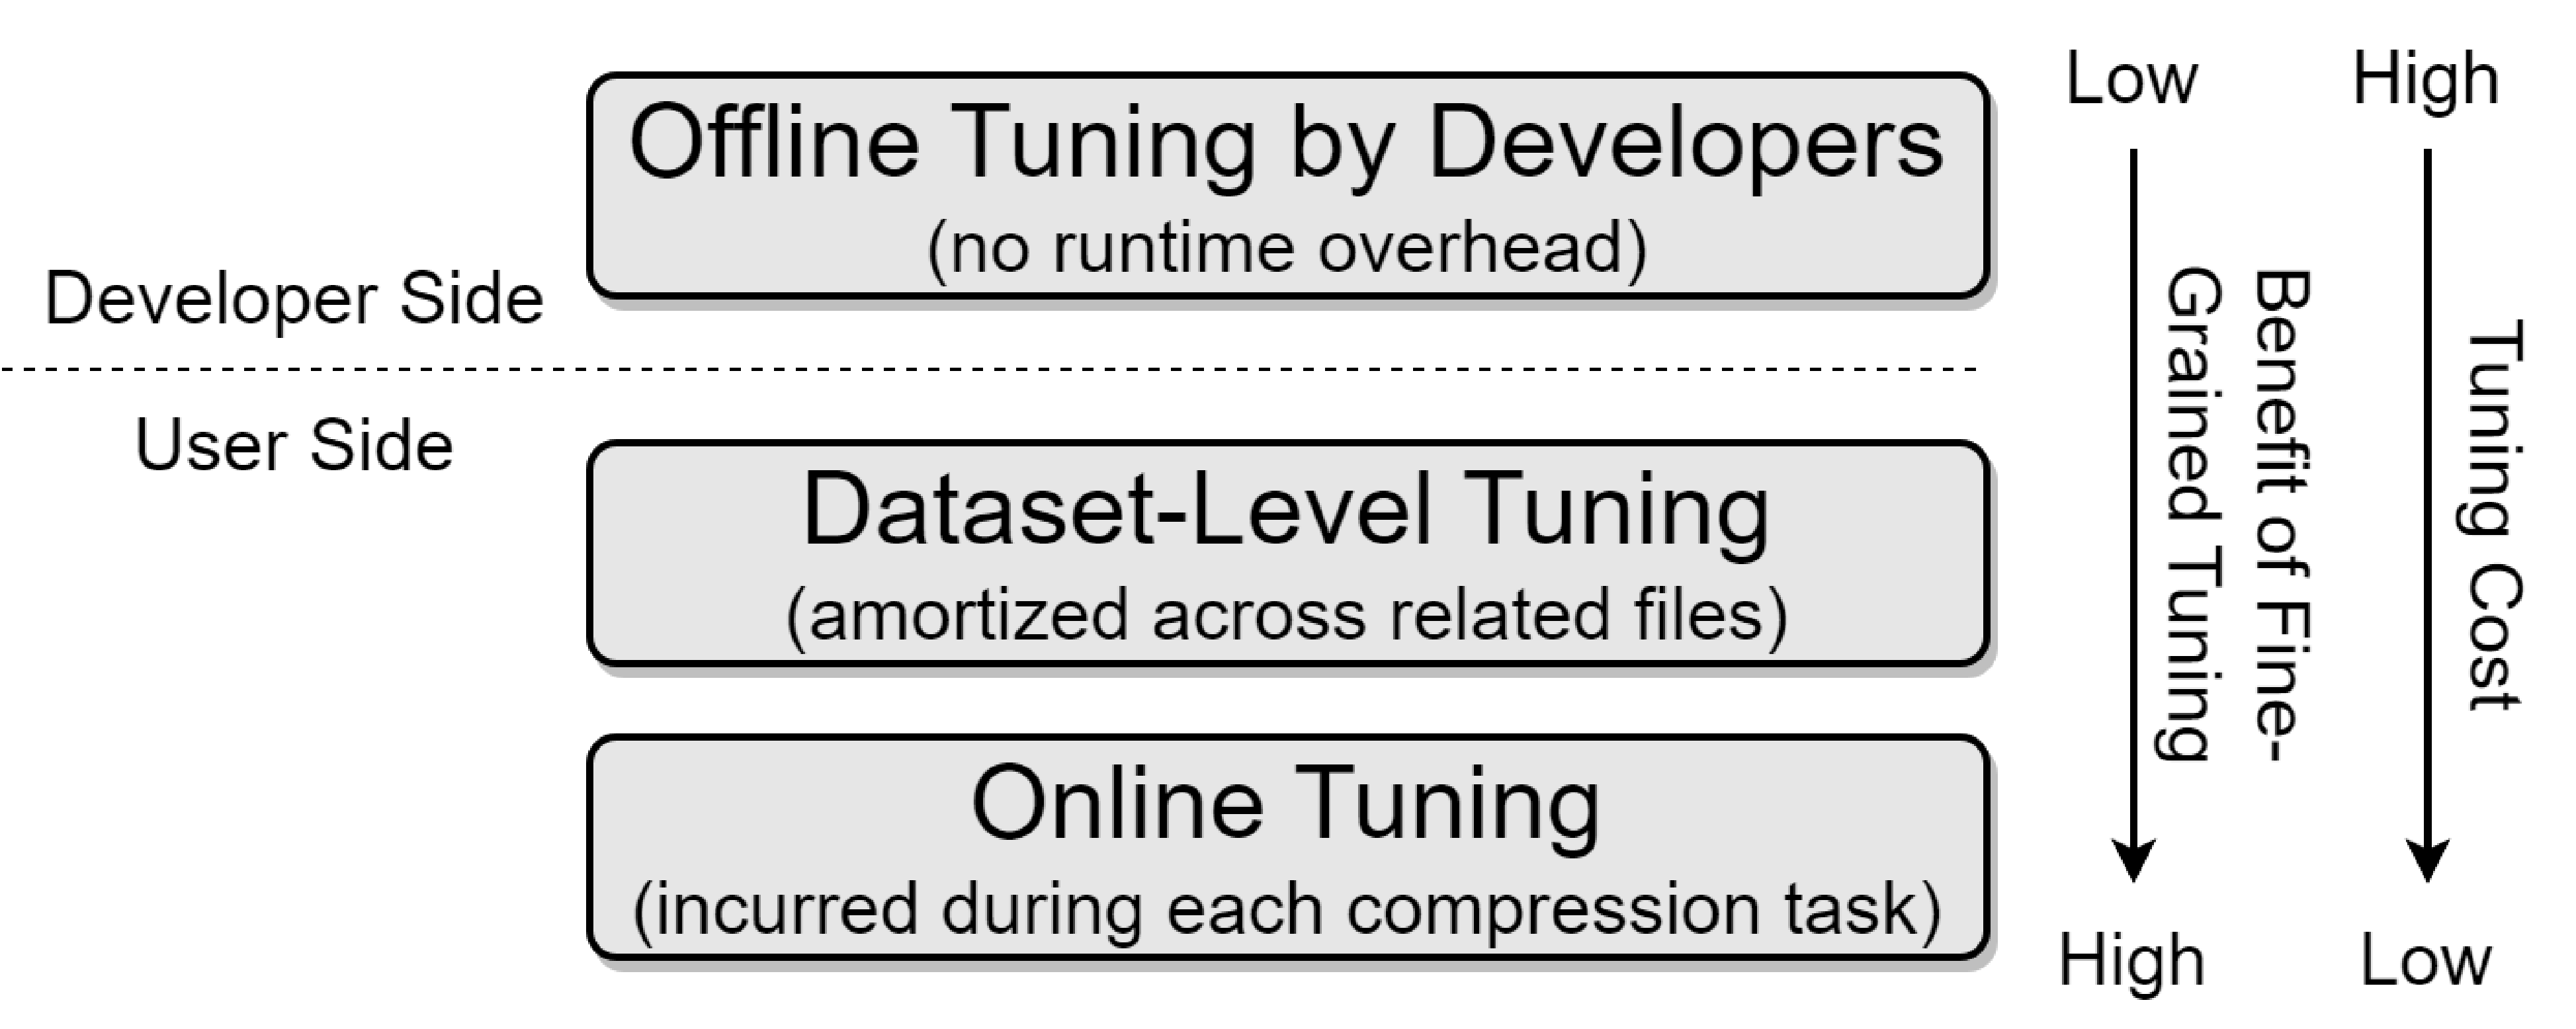
\includegraphics[width=0.7\linewidth]{figs/3/diagram1.pdf}
    \caption{Hierarchical Organization of Configuration Tuning}
    \label{fig:diagram1}
\end{figure}

Exploring all configuration dimensions uniformly at runtime is neither necessary nor practical. As illustrated in Figure~\ref{fig:diagram1}, we therefore assign different tuning steps to three stages: offline tuning performed by compressor developers across multiple datasets, dataset-level tuning performed before compression on representative data, and online tuning performed during compression for individual files or data blocks. Offline tuning introduces no runtime overhead for users, while dataset-level tuning costs can be amortized across related files. In contrast, online tuning costs are incurred during compression and must therefore remain sufficiently low.

The appropriate stage for each configuration dimension depends on its expected benefit and tuning cost. These two aspects are determined by several interrelated factors. We consider the following factors:

\begin{itemize}
\item \textbf{Regularity of the performance landscape} describes how smoothly and predictably compression performance changes as a numerical configuration varies while other configurations are fixed. If the response is smooth and approximately unimodal, a near-optimal value can often be identified using only a small number of evaluations. The regularity of the response may depend on the amount of data used for evaluation. Aggregating performance over an entire dataset or a large data region tends to average out local variations, whereas evaluation on a small data block may produce irregular fluctuations caused by its limited and highly localized data characteristics.

\item \textbf{Magnitude of the potential gain} describes the expected maximum performance improvement achievable through tuning relative to a fixed default choice. Dimensions with limited potential gains may not justify expensive or repeated tuning.

\item \textbf{Generalizability} describes whether a selected configuration can be reused across datasets or across related files, variables, or timesteps. Greater reuse allows the tuning overhead to be amortized over more compression tasks.

\item \textbf{Size of the candidate space} describes the number of possible choices and, consequently, the number of candidates that may need to be evaluated. For categorical or integer-valued configurations, the candidate space is explicitly defined. For continuous-valued configurations, however, its effective size depends on both the search range and the sampling resolution. The required resolution is further influenced by the regularity of the performance landscape and the magnitude of the potential tuning gain.

\item \textbf{Interaction with other configuration dimensions} describes the extent to which the best choice for one dimension depends on the choices made for other dimensions. Weakly interacting dimensions can be tuned independently or sequentially, while strongly interacting dimensions may require joint search.

\item \textbf{Availability and reliability of proxy metrics} describes whether candidate configurations can be evaluated without executing the complete compression pipeline. An inexpensive and sufficiently reliable proxy can enable fine-grained online tuning by reducing the per-candidate evaluation cost. However, a proxy that poorly preserves the relative ranking of candidates may lead to suboptimal decisions, even if it is inexpensive to compute.
\end{itemize}

These factors should be considered jointly rather than as independent assignment rules. Each factor indicates a tendency toward a particular tuning stage, so a configuration dimension may be suitable for more than one stage. The final assignment is therefore necessarily empirical and may involve trade-offs between data-specific adaptation and practical preprocessing and execution overhead.
\section{Tunable Dimensions in the SZ Compression Pipeline}\label{sec:tunable dimensions}

In this section, we first review the general workflow of the SZ compression pipeline. We then identify the tunable configuration dimensions exposed by this pipeline and analyze their potential benefits and tuning costs under the hierarchical framework introduced in Section~\ref{sec:framework}, with the goal of determining appropriate tuning stages for different dimensions.

\subsection{SZ Compression Pipeline}

\begin{figure}[htb]
    \centering
    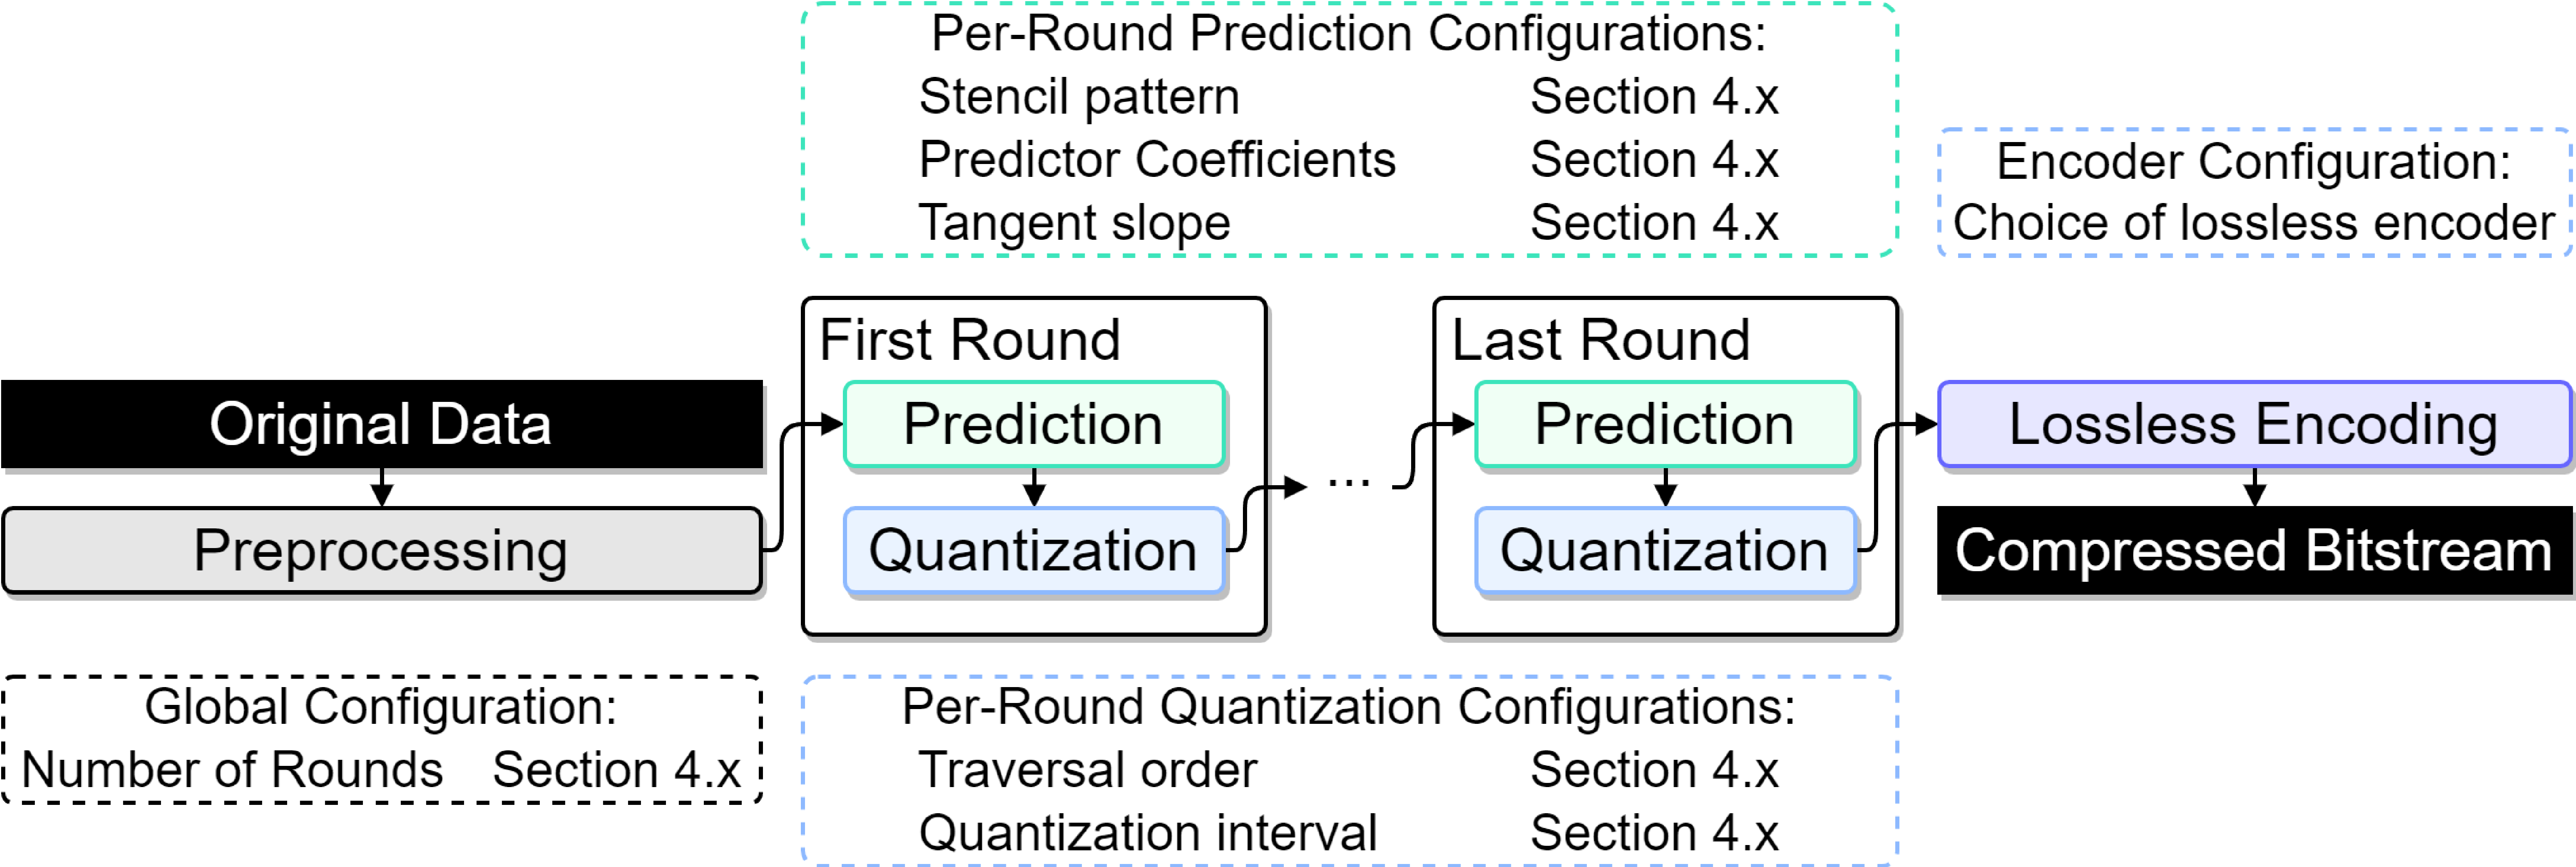
\includegraphics[width=1\linewidth]{figs/4/diagram2.pdf}
    \caption{Enter Caption}
    \label{fig:diagram2}
\end{figure}

The SZ compression pipeline mainly consists of three components: prediction, quantization of prediction residuals, and lossless encoding. As illustrated in Figure~\ref{fig:diagram2}, the prediction and quantization stages are divided into multiple rounds and executed iteratively. Each prediction round reconstructs a new set of data values, which can then serve as references in subsequent rounds. Lossless compression is applied only after the quantized residuals of all prediction rounds have been generated. The three components are described as follows.

\begin{itemize}
\item \textbf{Prediction.} A predictor commonly used in the SZ pipeline computes a weighted sum of selected reconstructed data points, referred to as \emph{reference points}, to estimate a data value that has not yet been reconstructed, referred to as the \emph{prediction target}. During decompression, the original data are unavailable, and the predictor can only access values that have already been reconstructed. Therefore, reference points must be selected exclusively from previously reconstructed data so that the compressor and decompressor can generate identical predictions. Such a weighted-sum predictor is characterized by a \emph{stencil pattern} and a set of \emph{coefficients}. The stencil pattern specifies the relative locations of the reference points with respect to the prediction target. The coefficients specify the weights assigned to the individual reference points.

Prediction is typically organized into multiple rounds. In each round, the number of newly predicted targets is approximately equal to the total number of values already reconstructed. Consequently, later rounds process progressively larger portions of the dataset and therefore have a substantially greater impact on the overall compression performance than earlier rounds.

\item \textbf{Quantization of prediction residuals.} For each prediction target, the compressor computes the difference between its original value and predicted value, and quantizes this residual to an integer multiple of the quantization interval $\Delta$. The quantized residual is then added to the prediction to obtain the reconstructed lossy value.

In the standard setting, choosing $\Delta=2\epsilon$, where $\epsilon$ is the user-specified error bound, guarantees pointwise error boundedness. However, a narrower quantization interval also preserves the error bound.

\item \textbf{Lossless compression.} After all prediction residuals have been quantized, the resulting integer symbols are losslessly encoded. Liu et al.~\cite{liu2021improving} showed that different lossless encoders can lead to different trade-offs between compression ratio and throughput. Their results indicate that Huffman coding followed by Zstandard compression provides moderate compression ratios while achieving the highest compression throughput. We therefore fix this encoding pipeline in ASZ and focus our configuration exploration on prediction and quantization.
\end{itemize}

\subsection{Tangent-Based Rate--Distortion Comparison}\label{sec:tunable dimensions:tangent}

The objective of error-bounded lossy compression is to achieve both a lower bit rate and higher reconstruction quality. However, a configuration change often introduces a trade-off between these two metrics: it may improve PSNR while increasing the bit rate, or reduce the bit rate at the cost of lower PSNR. Prior work by Liang et al.~\cite{liang2019significantly} compares configurations by adjusting their error bounds until they achieve the same bit rate or PSNR. Although this approach enables a direct comparison, it may require multiple additional compression runs.

\begin{figure}[htb]
    \centering
    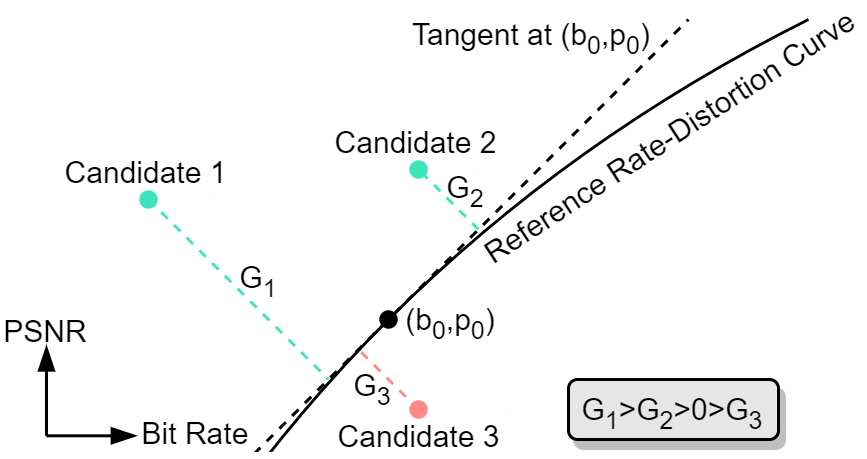
\includegraphics[width=0.7\linewidth]{figs/4/projection.png}
    \caption{Tangent-Based Rate--Distortion Comparison}
    \label{fig:tangent}
\end{figure}

To avoid this additional evaluation overhead, we propose a tangent-based rate--distortion comparison criterion, as illustrated in Figure~\ref{fig:tangent}. Given a reference configuration and a target error bound $eb_0$, we estimate the tangent of its rate--distortion curve at the corresponding operating point $(b_0,p_0)$, where $b_0$ denotes the bit rate and $p_0$ denotes PSNR. Specifically, we evaluate the reference configuration at two nearby error bounds on opposite sides of $eb_0$, namely, $eb_{\mathrm{low}}=eb_0/r$ and $eb_{\mathrm{high}}=eb_0r$, where $r>1$, obtaining the corresponding operating points $(b_{\mathrm{low}},p_{\mathrm{low}})$ and $(b_{\mathrm{high}},p_{\mathrm{high}})$. We approximate the local rate--distortion slope as
\begin{equation}
m_{\mathrm{RD}}=\frac{p_{\mathrm{high}}-p_{\mathrm{low}}}{b_{\mathrm{high}}-b_{\mathrm{low}}}.
\end{equation}

The estimated tangent at $(b_0,p_0)$ is expressed as
\begin{equation}
p-p_0=m_{\mathrm{RD}}(b-b_0).
\end{equation}

For a candidate configuration with operating point $(b_c,p_c)$ under the same error bound $eb_0$, we define its gain as the normalized signed offset from $(b_c,p_c)$ to the reference tangent:
\begin{equation}
G=\frac{p_c-p_0-m_{\mathrm{RD}}(b_c-b_0)}{\sqrt{1+m_{\mathrm{RD}}^2}}.
\end{equation}

A positive value of $G$ indicates that the candidate lies above the reference tangent, toward the preferred upper-left region of the rate--distortion plane, and therefore improves the local rate--distortion trade-off. $G=0$ indicates that the candidate moves only along the local rate--distortion trend. Therefore, candidates with larger values of $G$ are preferred.

\subsection{Analysis of Tunable Configuration Dimensions}\label{sec:tunable dimensions:analysis}

In the remainder of this section, we provide a more detailed explanation of the tunable configuration dimensions summarized in Figure~\ref{fig:diagram2}. For each dimension, we analyze its potential rate--distortion benefit, tuning costs and generalizability. Based on these factors, we determine the appropriate tuning stage within the hierarchical framework shown in Figure~\ref{fig:diagram1}. We first examine stencil patterns and predictor coefficients in Sections~\ref{aaa}---~\ref{bbb}, as these two dimensions are closely coupled and jointly determine the behavior of a predictor. We then analyze XXX.

\subsubsection{Tunable-Coefficient Predictors}\label{sec:tunable dimensions:analysis:TC predictor}\mbox{}

A weighted-sum predictor is jointly characterized by its stencil pattern and coefficients. The stencil pattern specifies the locations of the reference points relative to the prediction target, while the coefficients determine how these references are combined. In principle, a predictor may use reference points from a large neighborhood to exploit more information. In practice, however, only previously reconstructed values are available to both compression and decompression, and larger stencils increase computation costs. The stencil pattern therefore determines a restricted set of usable references.

\begin{figure}[htb]
    \centering
    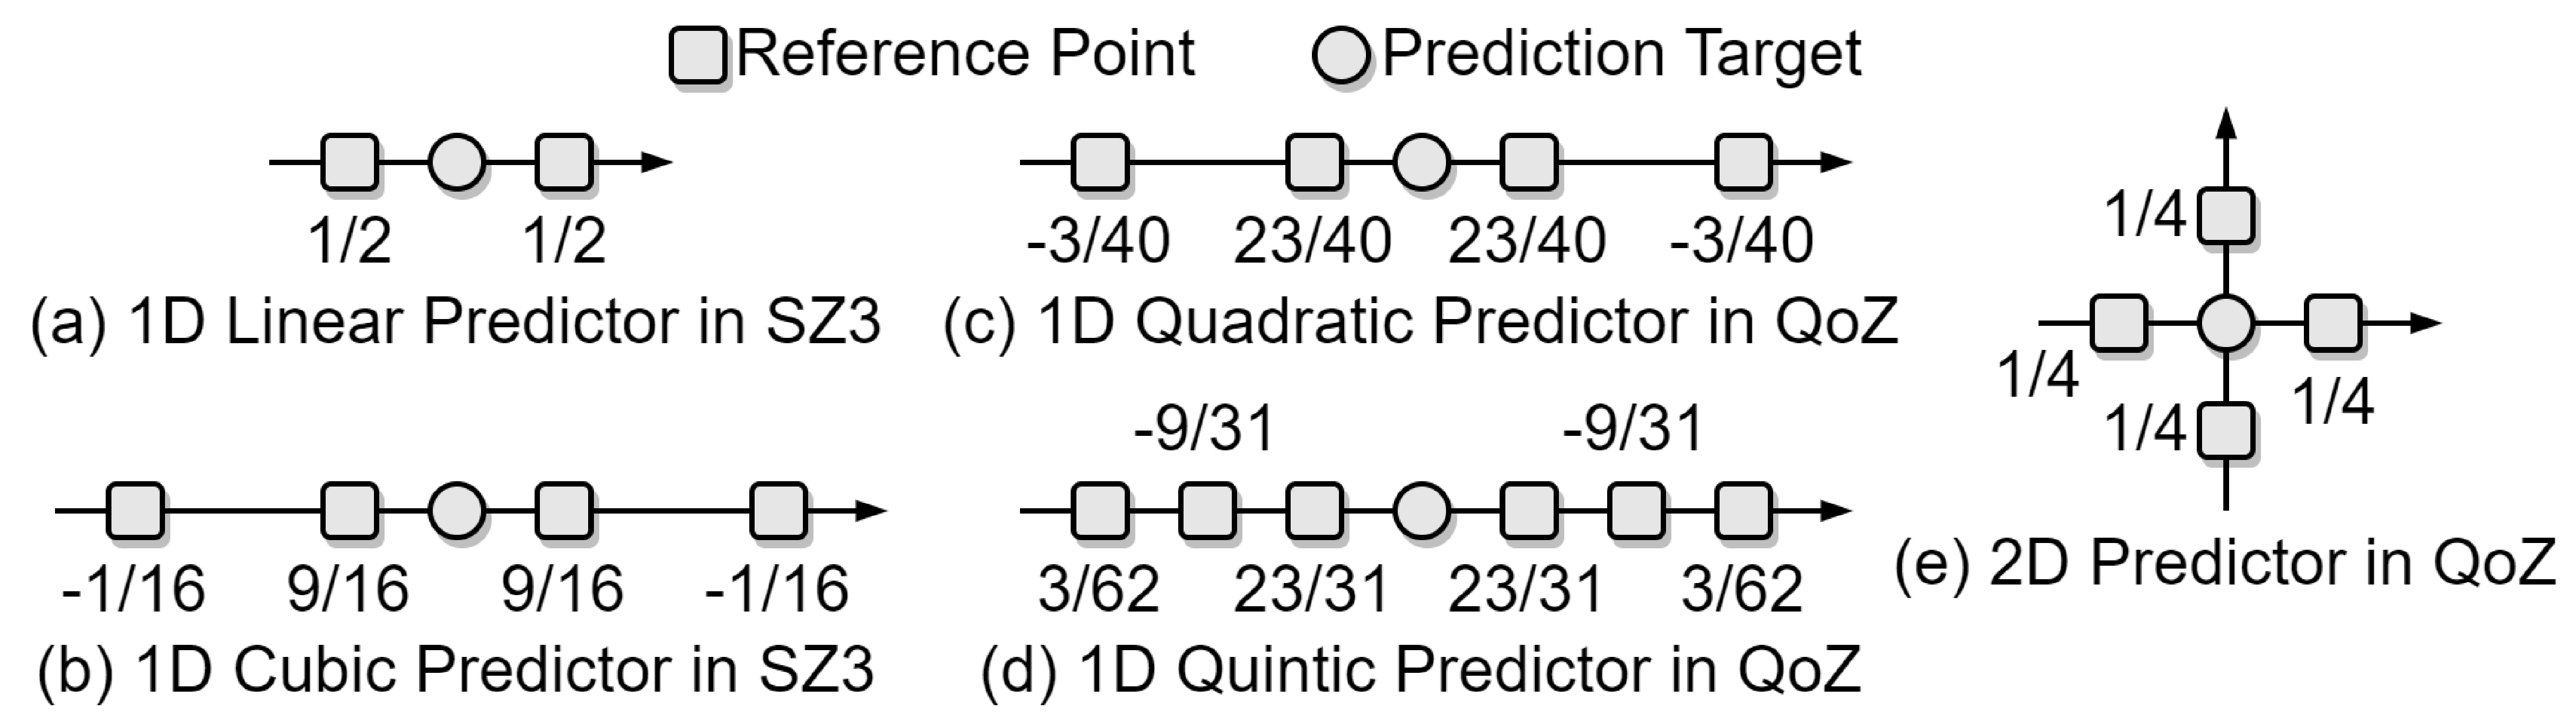
\includegraphics[width=1\linewidth]{figs/4/stencil patterns.pdf}
    \caption{Enter Caption}
    \label{fig:sp}
\end{figure}

Figure~\ref{fig:sp} illustrates several predictors used in SZ3 and QoZ. Additional predictors can be obtained by rotating these stencil patterns to align with different spatial dimensions. 

Both compressors include a predictor with four reference points along the same line (1D cubic predictor in SZ3 and 1D quadratic predictor in QoZ). However, they assign different coefficients to the same stencil pattern because they make different assumptions about local data behavior. SZ3 derives its coefficients by fitting a cubic polynomial through the four reference points, whereas QoZ constructs a piecewise quadratic spline under zero-slope boundary conditions. Other assumptions about local data characteristics can lead to different coefficient assignments. For example, under a stationary AR(1) correlation model, as the correlation parameter increases from $0$ toward $1$, the MSE-optimal coefficient assigned to each of the two reference points nearest to the prediction target increases from $0.25$ toward $0.5$. Meanwhile, the coefficients of the two outer reference points decrease from $0.25$ toward $0$. Notably, the coefficients assigned to the two inner reference points by SZ3 and QoZ are both greater than $0.5$, and therefore cannot be obtained under this stationary AR(1) model for any correlation parameter in $[0,1)$. These examples indicate that different assumptions about local data behavior lead to substantially different coefficient assignments, and no fixed coefficient assignment is uniformly optimal across different data characteristics.

Motivated by this observation, we define a ``tunable-coefficient predictor'' as a predictor with a fixed stencil pattern but adjustable coefficients. We constrain the coefficients to sum to one so that the prediction is exact for constant-valued data. Since all stencil patterns considered in this work are symmetric, coefficients at symmetric reference locations are constrained to be equal. When evaluating a tunable-coefficient predictor, we uniformly sample the feasible coefficient space and report the coefficient assignment that performs best under the tangent-based rate--distortion criterion introduced in Section~\ref{sec:tunable dimensions:tangent}.

\begin{figure}
    \centering
    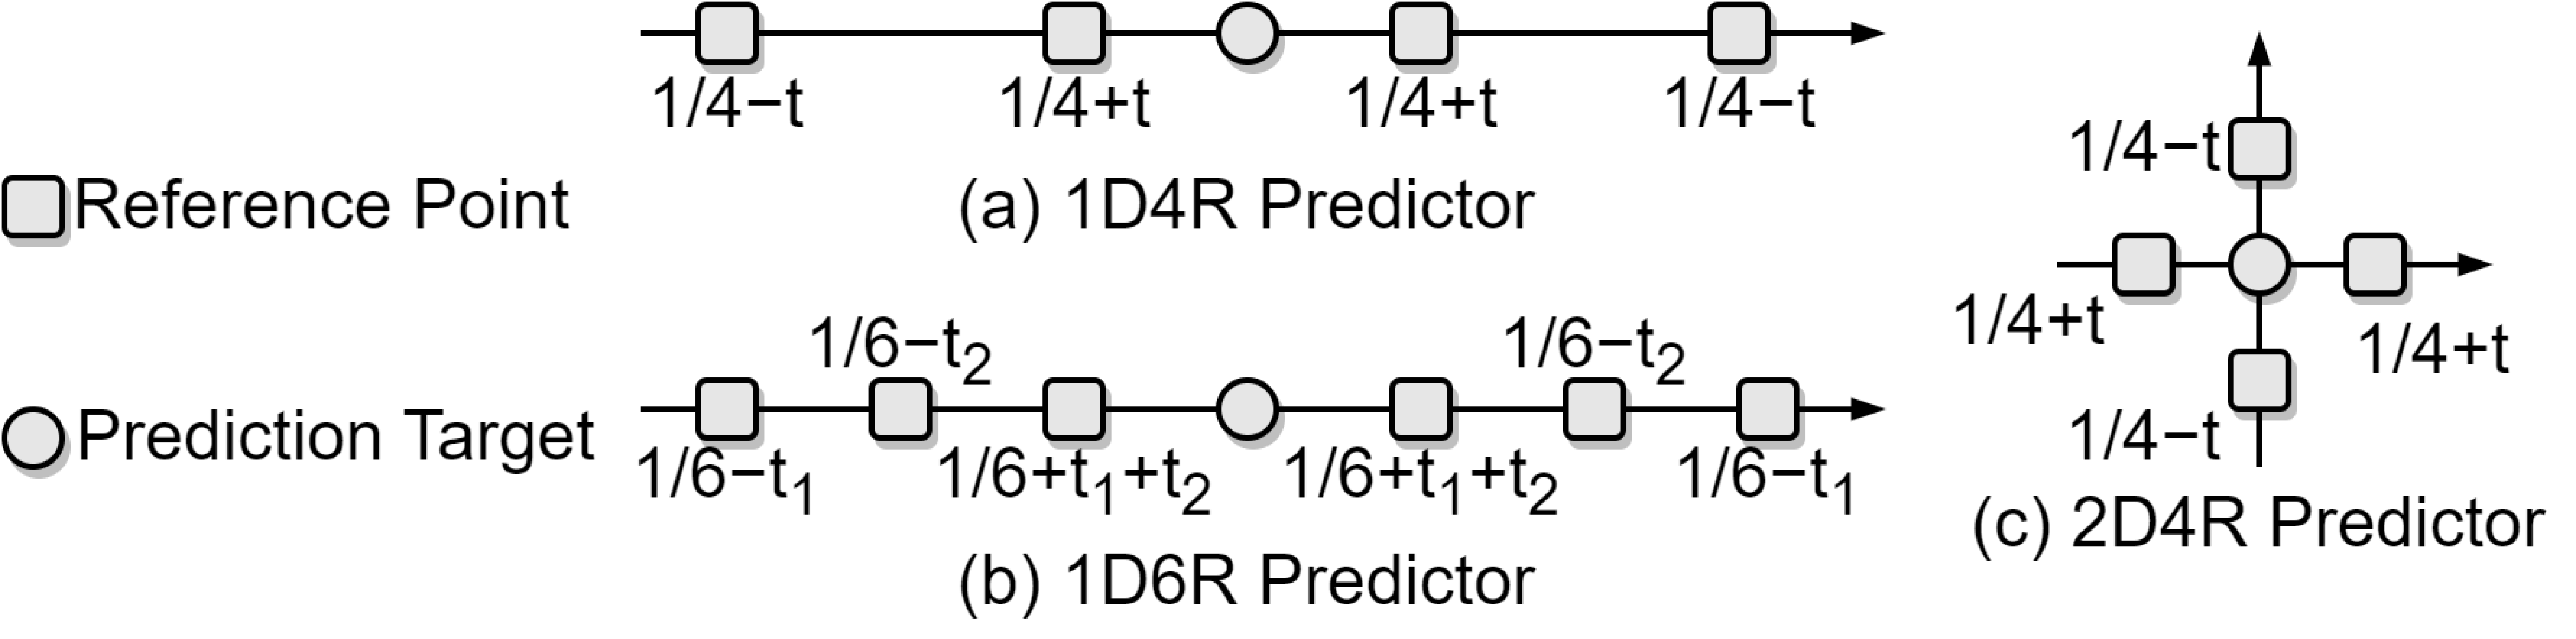
\includegraphics[width=1\linewidth]{figs/4/tunable coefficient stencil patterns.pdf}
    \caption{Enter Caption}
    \label{fig:tcsp}
\end{figure}

Predictors obtained by orienting the stencil geometry along different spatial directions form a predictor family. Figure~\ref{fig:tcsp} illustrates the three tunable-coefficient predictor families considered in this work. We use the notation $X$D$Y$R to denote a family whose predictors use $Y$ reference points distributed across $X$ spatial dimensions. 1D4R predictor family generalizes the linear and cubic predictors in SZ3 and the quadratic predictor in QoZ. Similarly, the 2D4R family generalizes the 2D predictor in QoZ, while the 1D6R family generalizes the quintic predictor in QoZ.

We evaluate the three tunable-coefficient predictor families on the ISABEL and CLDICE datasets in Table~\ref{tab:datasets}, and report their rate--distortion performance in Figure~\ref{fig:compare sp}. Both datasets are three-dimensional. Therefore, each predictor family can be instantiated along three orientations, corresponding to the three curves of the same color. The results lead to two main observations.

\begin{figure}[htb]
    \centering
    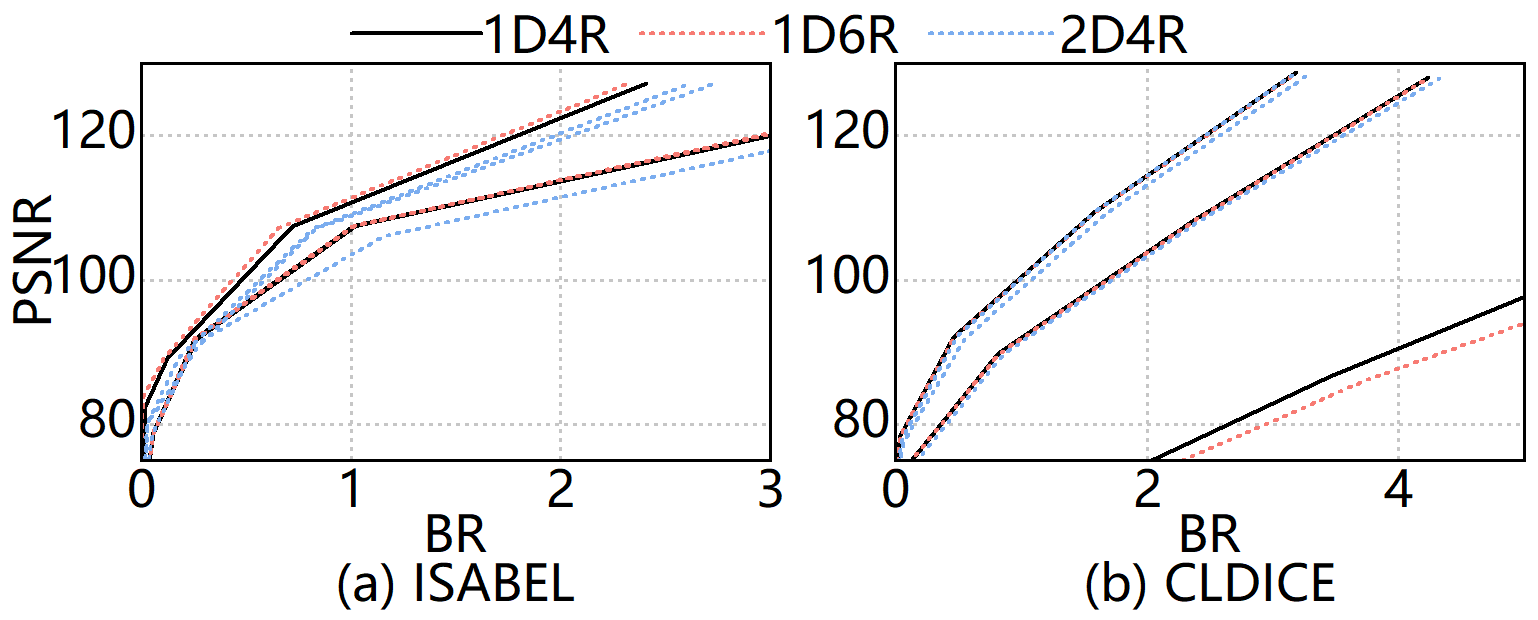
\includegraphics[width=0.8\linewidth]{figs/4/比较stencil pattern.png}
    \caption{Enter Caption}
    \label{fig:compare sp}
\end{figure}

\begin{itemize}
\item \textbf{The 2D4R predictors consistently underperform the 1D4R predictors.} After coefficient tuning, a 1D4R predictor can adaptively determine how much local nonlinear variation around the prediction target should be exploited. On noisy data, this information is often unreliable, and the optimal coefficients tend to approach those of the linear predictor in SZ3. On smoother data, the optimal coefficients tend to move toward those of the cubic predictor in SZ3 or the quadratic predictor in QoZ. This behavior suggests that the preferred 1D4R coefficients primarily reflect the overall usefulness of local nonlinear information, which is strongly influenced by the noise level and is often relatively consistent across a dataset.

In contrast, a 2D4R predictor can be viewed as a weighted combination of two one-dimensional linear predictions along different dimensions. Since neither component captures local nonlinear information, the resulting prediction errors contain unresolved nonlinear components from both directions. Appropriate coefficients may partially cancel these errors, but such cancellation is highly dependent on local data behavior and therefore does not generalize well across the dataset. This provides a possible explanation for the consistently weaker performance of 2D4R predictors.

\item \textbf{The improvement of 1D6R over 1D4R is very limited.} As shown in Figure~\ref{fig:compare sp}, the difference between the best 1D6R and 1D4R predictors is substantially smaller than the difference between the three oriented 1D4R predictors. Moreover, 1D6R introduces a larger coefficient-search space and incurs slightly higher prediction cost because it uses more reference points. We therefore exclude both 2D4R and 1D6R from the subsequent tuning space and retain 1D4R as the tunable-coefficient predictor family used in ASZ.
% 补充一下1D4R的参数搜索空间其实是1D6R的子集，所以最好的1D6R一定比最好的1D4R更好，但是优势非常少。
\end{itemize}

\subsubsection{Tuning Sequence of Stencil Patterns}\mbox{}

Existing compressors have explored tuning stencil patterns across prediction rounds, but only within restricted sequence structures. For three-dimensional data, SZ3 organizes every three consecutive rounds into a group, with the three rounds performing one-dimensional prediction along the three spatial dimensions, respectively. The prediction directions can be reordered within a group, but the same order is reused across all groups. QoZ expands this design by introducing two-dimensional predictors and allowing different groups to use different prediction orders. Nevertheless, both approaches retain the group structure and therefore explore only a restricted subset of possible prediction sequences.

We remove this grouping constraint and allow the differently oriented 1D4R predictors to be arranged freely across prediction rounds. The resulting search space grows exponentially with the number of rounds, making exhaustive evaluation impractical. We therefore adopt a backward greedy strategy that prioritizes the later prediction rounds. Specifically, we first select the stencil pattern for the final round and then proceed backward through the preceding rounds. Later rounds process substantially more prediction targets than earlier rounds and therefore generally have a greater impact on the overall rate--distortion performance. By fixing these high-impact choices first, the backward search provides an efficient approximation to exhaustive sequence tuning.

\begin{figure}[htb]
    \centering
    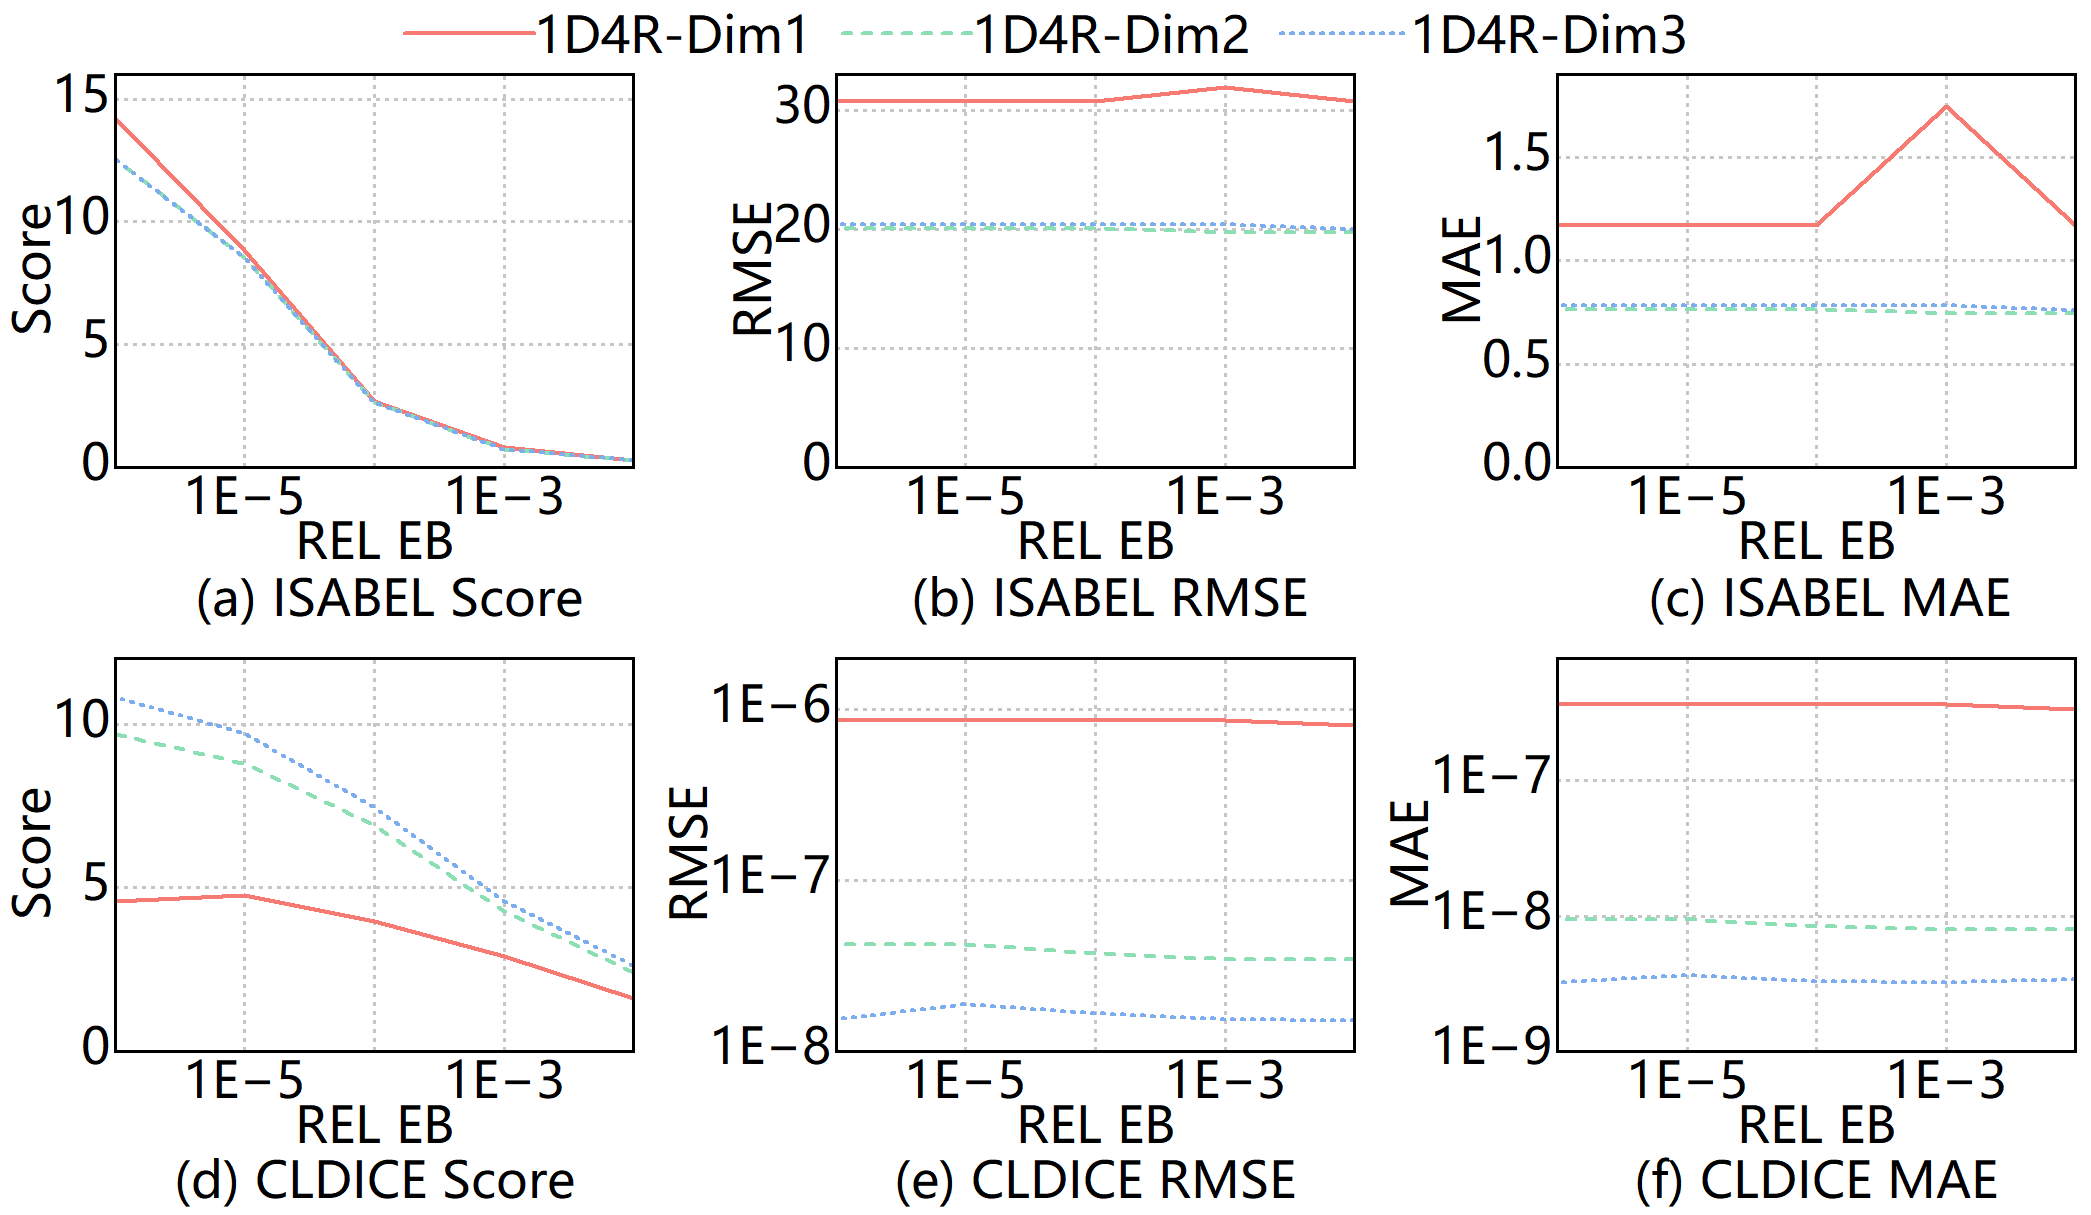
\includegraphics[width=1\linewidth]{figs/4/检验stencil pattern的proxy.png}
    \caption{Enter Caption}
    \label{fig:verify sp proxy}
\end{figure}

By comparing the solid black curves in Figure~\ref{fig:compare sp}, we observe that tuning the stencil pattern can provide significant rate--distortion improvement. However, we do not identify a reliable proxy for accelerating this tuning process.
Figure~\ref{fig:verify sp proxy} compares the tangent-based bit-rate--PSNR scores, prediction RMSE, and prediction MAE of the 1D4R predictors oriented along the three spatial dimensions on the ISABEL and CLDICE datasets. In principle, a well-performing predictor is expected to achieve a high rate--distortion score together with low prediction RMSE and MAE. However, this relationship is not consistently observed. On ISABEL, the predictor oriented along the first dimension achieves a high rate--distortion score despite also exhibiting high RMSE and MAE. Consequently, neither RMSE nor MAE reliably preserves the ranking of stencil candidates and therefore cannot serve as an effective proxy for stencil-pattern tuning. We further discuss the cause of this discrepancy in Section~\ref{sec:discussion}.

% 还要验证跨文件普适性

\subsubsection{Tuning Coefficients}\mbox{}

After selecting a 1D4R predictor, we further examine whether tuning its coefficients provides meaningful rate--distortion improvement. On the ISABEL and CLDICE datasets, we apply the best-performing 1D4R predictor identified in the preceding analysis and vary only its coefficient assignment. Figure~\ref{fig:bbb} compares the resulting rate--distortion curves.

The results show that different coefficient assignments can lead to substantial differences in rate--distortion performance. Moreover, the best-performing coefficients vary across datasets and error bounds, confirming that no single fixed assignment consistently achieves the best performance.

Predictor coefficients interact strongly with stencil patterns. Within the 1D4R family, predictors oriented along different dimensions may favor different coefficient assignments because the data can exhibit different characteristics along these dimensions. Therefore, when tuning stencil patterns, we must first identify the best coefficient assignment for each stencil candidate before comparing their rate--distortion performance. Since this process requires repeated evaluation of coefficient candidates, reducing the cost of each evaluation is essential for efficient stencil-pattern tuning.

\begin{figure}[htb]
    \centering
    \includegraphics[width=0.8\linewidth]{bbb}
    \caption{bbb}
    \label{fig:bbb}
\end{figure}

To reduce this cost, we replace the tangent-based bit-rate--PSNR comparison introduced in Section~\ref{sec:tunable-dimensions-tangent} with an $H_1$--PSNR comparison when ranking coefficient assignments for the same stencil predictor. Here, $H_1$ denotes the first-order entropy of the quantized prediction residuals and serves as an estimate of the bit rate. As shown in the first two columns of Figure~\ref{fig:bbb}, replacing bit rate with $H_1$ largely preserves the relative positions of the curves produced by different coefficient assignments, indicating that the $H_1$--PSNR comparison approximates the ranking obtained by the bit-rate--PSNR comparison.

The third column of Figure~\ref{fig:bbb} compares the ranking accuracy of five inexpensive evaluation criteria: the proposed $H_1$--PSNR criterion, $H_1$ alone, PSNR alone, prediction MSE, and prediction MAE. The horizontal axis shows the relative error bound, while the vertical axis reports Kendall's $\tau$ between the candidate ranking produced by each criterion and the ranking produced by the bit-rate--PSNR criterion. Across the evaluated error bounds, the $H_1$--PSNR criterion achieves the highest ranking accuracy.

Compared with the original bit-rate--PSNR criterion, the $H_1$--PSNR criterion first reduces the evaluation cost by eliminating lossless encoding. Both $H_1$ and PSNR can be obtained while computing the quantized prediction errors: $H_1$ is calculated from the resulting symbol distribution, while PSNR is derived from the corresponding reconstruction errors.

A direct evaluation of the $H_1$--PSNR criterion processes each coefficient candidate independently. For each candidate, it predicts all sampled target values, quantizes the resulting prediction errors, counts the frequencies of the quantization symbols to compute $H_1$, and accumulates the reconstruction errors to compute PSNR. Although this approach avoids the lossless-encoding stage required by the bit-rate--PSNR criterion, it still requires prediction and quantization for every combination of coefficient candidate and sampled target.

The evaluation can be further accelerated without explicitly computing and quantizing the prediction error of every sampled target for every coefficient candidate. Both $H_1$ and PSNR depend only on the distribution of prediction errors, rather than on their spatial ordering. Therefore, once an accurate approximation of this distribution is available, the frequencies of the quantized prediction-error symbols and the resulting PSNR can be estimated directly using the following equations.

Let the prediction error $E$ follow a probability density function $f_E(e)$, and let $\Delta$ denote the quantization step size. Under uniform quantization, the probability of quantization symbol $i$ is
\begin{equation}
p_i=\int_{\left(i-\frac{1}{2}\right)\Delta}^{\left(i+\frac{1}{2}\right)\Delta}f_E(e)\,de.
\end{equation}
The first-order entropy is then computed as
\begin{equation}
H_1=-\sum_i p_i\log_2p_i.
\end{equation}
Because an error in the $i$th interval is reconstructed as $i\Delta$, the resulting mean squared reconstruction error is
\begin{equation}
\mathrm{MSE}_{\mathrm{rec}}=\sum_{i=-\infty}^{\infty}\int_{\left(i-\frac{1}{2}\right)\Delta}^{\left(i+\frac{1}{2}\right)\Delta}f_E(e)\left(e-i\Delta\right)^2\,de.
\end{equation}
The corresponding PSNR is
\begin{equation}
\mathrm{PSNR}=10\log_{10}\left(\frac{R^2}{\mathrm{MSE}_{\mathrm{rec}}}\right),
\end{equation}
where $R$ is the value range of the original data.


为了快速算出预测误差的分布，We exploit this property by expressing the prediction error as an affine function of the tunable coefficient. For the 1D4R predictor shown in Figure~\ref{fig:tcsp}, the prediction error for a target $x_0$ can be written as
\begin{equation}
e(t)=x_0-\left[\left(\frac{1}{4}-t\right)x_{-3}
+\left(\frac{1}{4}+t\right)x_{-1}
+\left(\frac{1}{4}+t\right)x_1
+\left(\frac{1}{4}-t\right)x_3\right]
=At+B,
\end{equation}
where
\begin{equation}
A=x_{-3}-x_{-1}-x_1+x_3
\end{equation}
and
\begin{equation}
B=x_0-\frac{x_{-3}+x_{-1}+x_1+x_3}{4}.
\end{equation}

The values of $A$ and $B$ are independent of the coefficient candidate $t$. We therefore compute them once for all sampled prediction targets and construct an approximate joint histogram of $(A,B)$. For a candidate $t$, each occupied histogram bin centered at $(a_j,b_j)$ is mapped to the prediction error $a_jt+b_j$. After quantizing these errors under the target error bound and aggregating the corresponding bin frequencies, we directly obtain an approximation of the quantized-error distribution used to compute $H_1$ and PSNR. This avoids recomputing the prediction error separately for every sampled target and every coefficient candidate.

Let $n$ be the number of sampled prediction targets, $k$ the number of coefficient candidates, and $h$ the number of occupied bins in the joint histogram of $(A,B)$. Direct evaluation computes an error for every target--candidate pair and therefore requires $O(kn)$ time. The histogram-based method requires $O(n)$ time to construct the joint histogram and $O(kh)$ time to evaluate all candidates, resulting in a total complexity of $O(n+kh)$. Since $h$ is typically much smaller than $n$, the evaluation cost is close to linear in the sample size.

The joint histogram need not preserve $A$ and $B$ at full numerical precision. The final $H_1$ calculation only distinguishes prediction errors after quantization, whose interval is determined by the error bound. Therefore, the discretization intervals used for $A$ and $B$ can be substantially smaller than, but need not be comparable to machine precision relative to, the final prediction-error quantization interval. In our implementation, setting their induced error uncertainty to a small fraction of the final quantization interval, such as $10\%$, is sufficient to preserve an accurate quantized-error distribution.

Moreover, the expressions for $A$ and $B$ represent local differences and interpolation residuals, respectively, and are therefore typically concentrated near zero for locally correlated scientific data. As a result, only a limited number of joint-histogram bins are occupied in practice, making $h\ll n$ and reducing the overall evaluation cost to approximately $O(n)$ for a fixed set of coefficient candidates.
\section{Design of ASZ}

\subsection{Overview}

\subsection{Offline Design-Space Exploration}

\subsection{Dataset-Level Dependency-Sequence Tuning}

\subsection{Dataset-Level Traversal-Order Tuning}

\subsection{Efficient Block-Level Coefficient Tuning}

\subsection{Overall Algorithm and Complexity}
% 加上generalizability的测试

\section{Performance Evaluation}\label{sec:performance}

This section evaluates the proposed compressors ASZ on datasets from different domains. We assess the effectiveness of ASZ from multiple perspectives, including data distortion, compressibility and compression throughput, and compare them against several state-of-the-art error-bounded lossy compressors.

\subsection{Experimental Setup}\label{sec:performance:setup}

\subsubsection{Evaluation Platform}
All experiments were conducted on [Supercomputer A]\footnote{Details are hidden due to the double-blind policy.} with one AMD EPYC 7763 64-Core processor used.
ASZ is compiled using GCC 11.2.0 using \verb|-Ofast| and \verb|-mavx2|, while baseline compressors were built separately using their default configuration.

\subsubsection{Datasets}

Table~\ref{tab:datasets} summarizes the datasets used in our evaluation. They originate from multiple domains and include scientific simulation data, real-world measurements, and data used in neural networks.

\begin{table}[htb]
    \centering
    \caption{Overview of Datasets}
    \label{tab:datasets}
    \setlength{\tabcolsep}{4pt}
    \begin{tabular}{lc|lc}
        \toprule
        Dataset    & Shape                      & Dataset & Shape \\
        \midrule
        Videollava & $8\times257\times4096$     & XPCS    & $998\times128\times128$ \\
        ISABEL     & $100\times500\times500$    & Aramco  & $449\times449\times235$ \\
        LETKF      & $98\times1200\times1200$   & CLDICE  & $26\times1800\times3600$ \\
        APSU004    & $1024\times1558\times1813$ & E017    & $1024\times1813\times1558$ \\
        \bottomrule
    \end{tabular}
\end{table}

\subsubsection{Baseline Compressors}

We use SZ3~\cite{liang2022sz3,zhao2021optimizing} and QoZ~\cite{liu2022dynamic,liu2024high} as baseline compressors in our evaluation. Both are state-of-the-art prediction-based error-bounded lossy compressors built upon the SZ compression framework and are discussed in Sections~\ref{sec:related work} and \ref{sec:preliminary study}. Since ASZ is also built upon the SZ compression framework, these two compressors provide the most relevant baselines for evaluating the effectiveness of our proposed techniques.

\subsection{Rate-Distortion Results}

We present the rate-distortion curves for all datasets in Table~\ref{tab:datasets} across all compressors. The X-axis shows the bitrate, and the Y-axis shows PSNR, a key metric for data quality. These curves capture the tradeoff between compressibility and reconstruction quality, with better performance indicated by points closer to the upper-left.

\begin{figure}[htb]
    \centering
    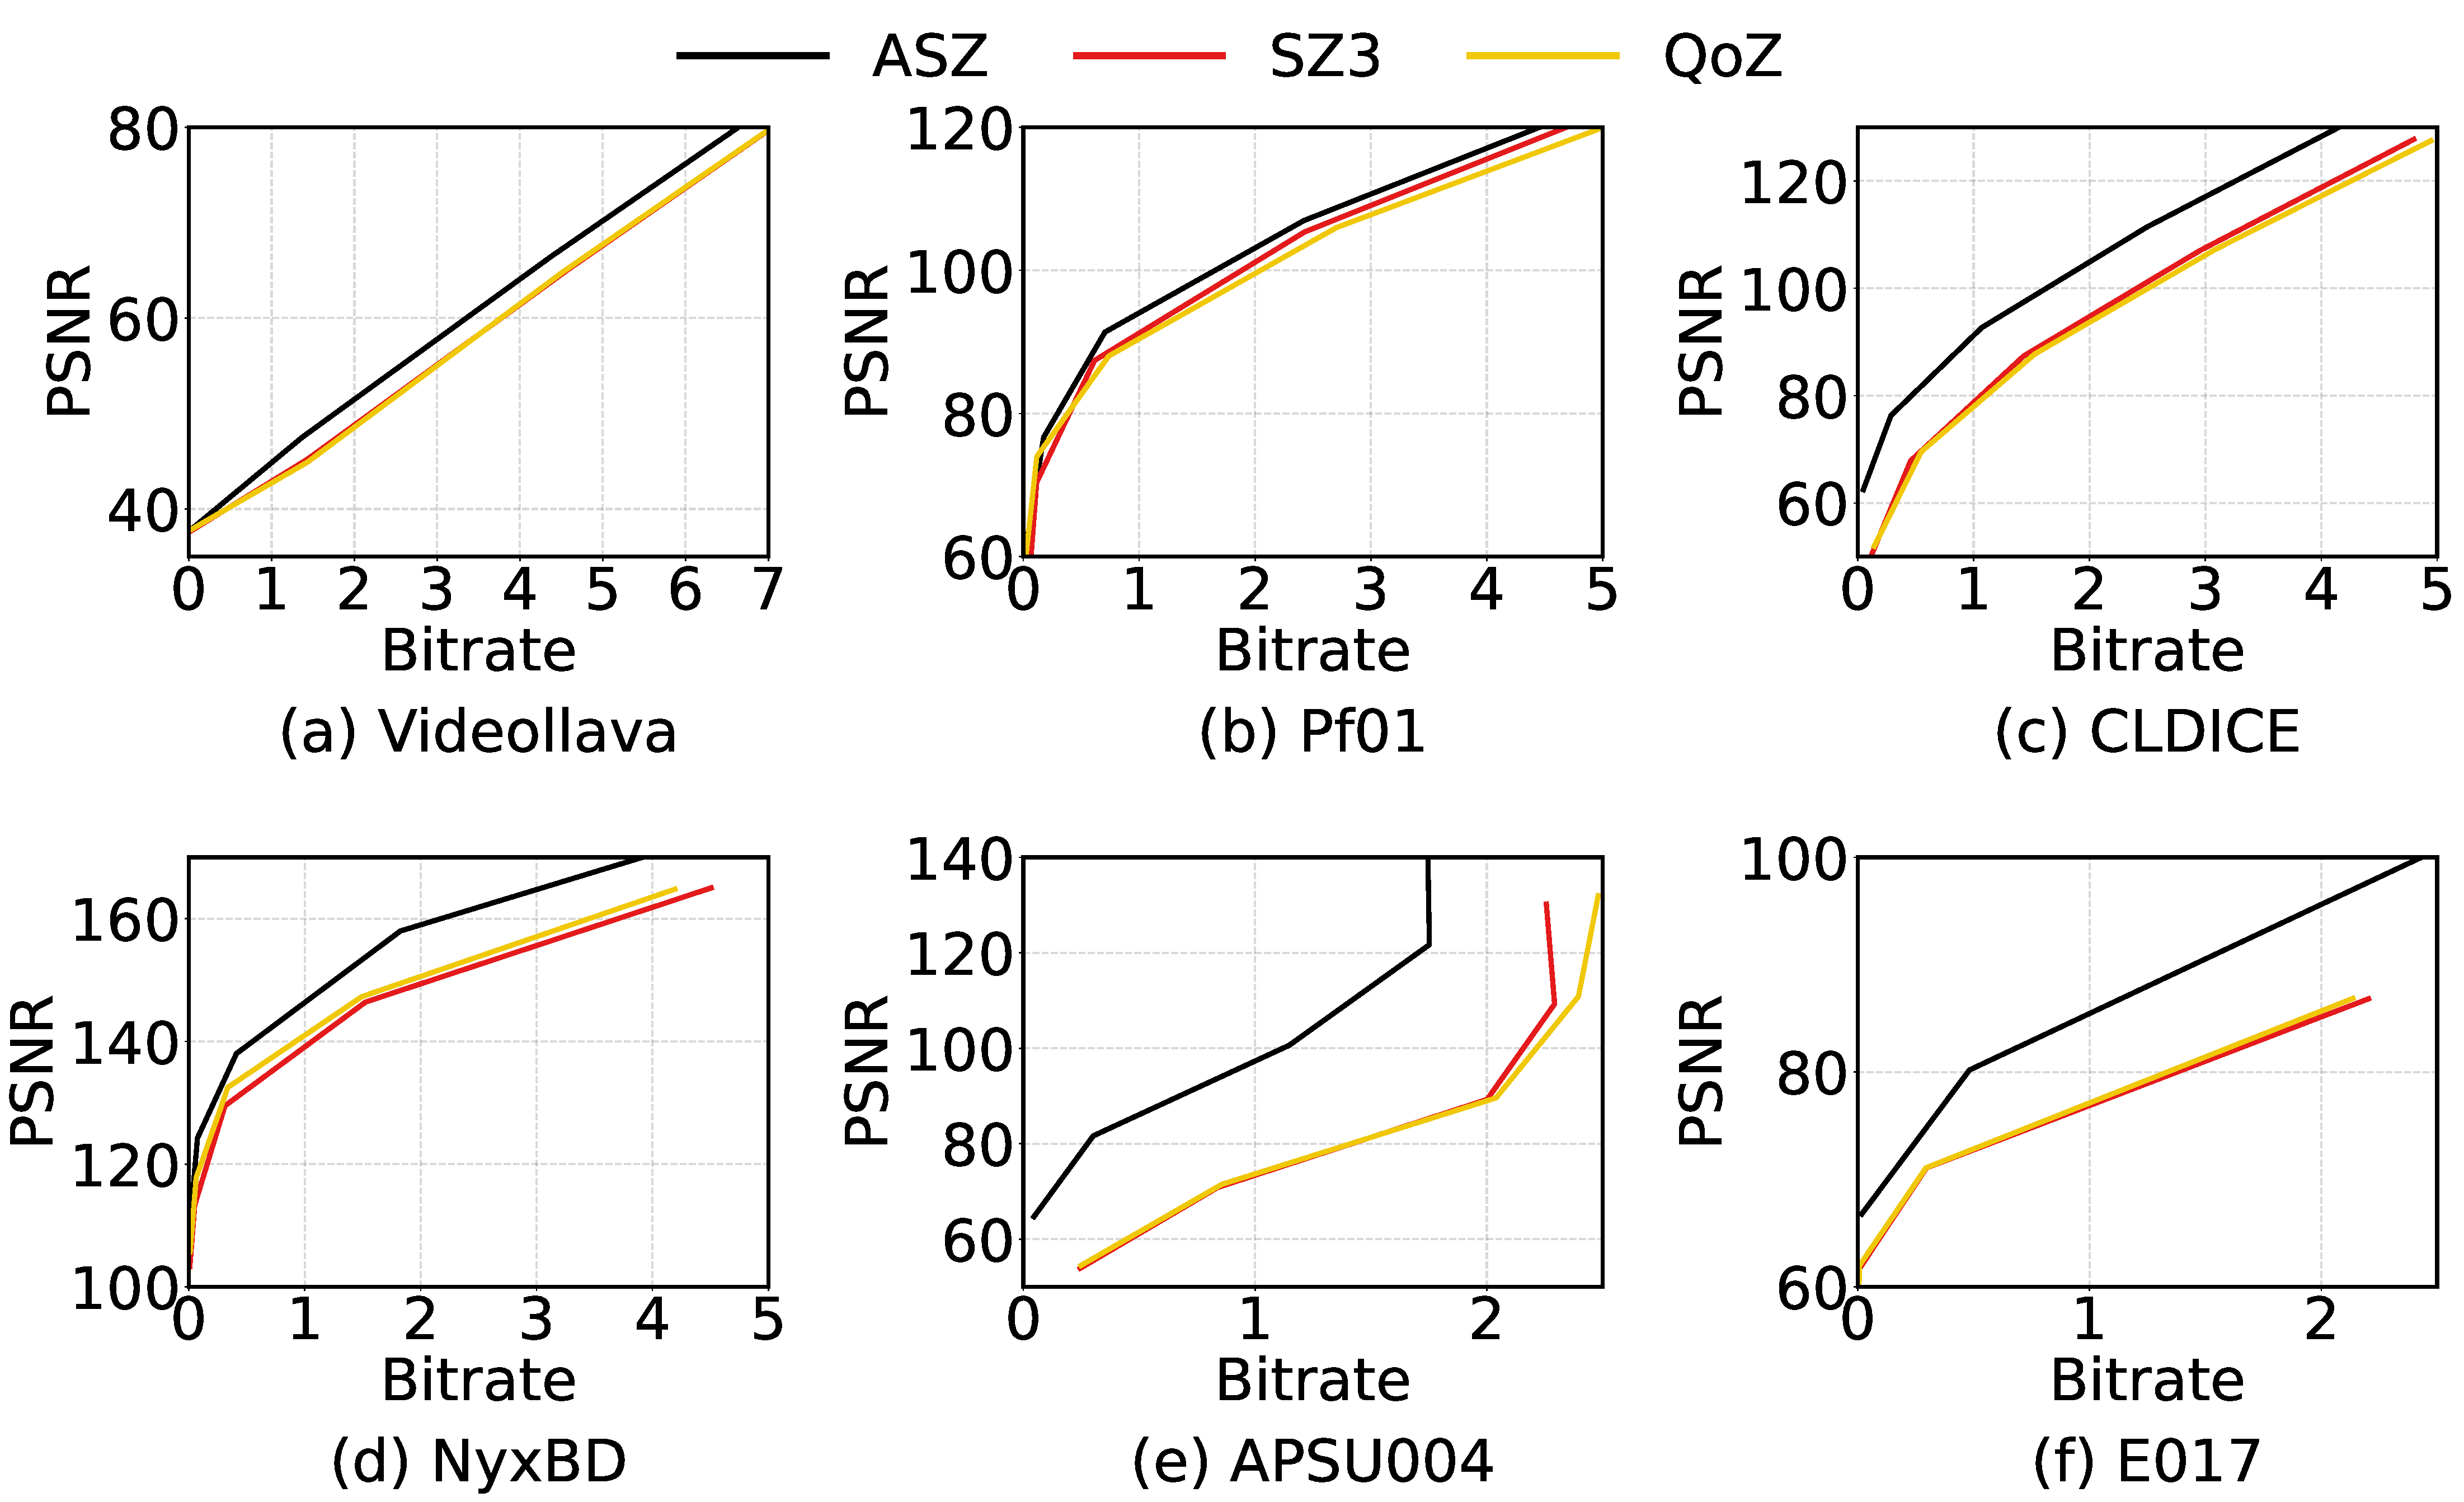
\includegraphics[width=1\linewidth]{figs/5/rate-distortion.pdf}
    \caption{Evaluation of rate-distortion curves between ASZ and baseline compressors}
    \label{fig:rate-distortion}
\end{figure}

Figure~\ref{fig:rate-distortion} presents the rate-distortion results. Overall, \textbf{\textit{ASZ consistently outperforms all baseline compressors across all evaluated datasets and error bounds}}. Under the same PSNR, ASZ can usually achieve $2\times$ higher compression ratio than the baseline compressors. Meanwhile, it shows particularly strong performance in two scenarios.

First, \textbf{\textit{ASZ shows particularly strong performance under large error bounds}}. Existing compressors, such as SZ3, typically switch between linear interpolation prediction under large error bounds and cubic interpolation prediction under small error bounds.  However, the predictor behavior in the medium-error-bound regime has not been systematically studied. ASZ addresses this issue by using higher-granularity coefficient tuning according to the local data characteristics and target error bound, enabling more accurate prediction and improved compression performance.

Second, \textbf{\textit{ASZ achieves especially large improvements on certain datasets}}, represented by APSU004, where ASZ can provide more than $60$\,dB higher PSNR under the same bitrate, or over $10\times$ higher compression ratio under the same PSNR compared with baseline compressors. For these datasets, one dimension is significantly more predictable than the others. ASZ is able to completely disable predictors along less predictable dimensions and rely only on the dominant predictive direction. In contrast, existing baseline compressors lack such adaptive predictor selection capability and therefore cannot fully exploit this type of anisotropic predictability.

\subsection{Compression Performance Breakdown}

% First, summarize what you will discuss.
In this section, we conduct ablation studies to evaluate the contribution of the major components in ASZ. We focus on three key mechanisms that distinguish ASZ from the traditional SZ compression framework:

\begin{itemize}
\item ASZ estimates the tangent of the rate-distortion curve and evaluates predictors by their displacement along the normal direction. As comparisons, we additionally evaluate two special cases where the tangent direction is set to be parallel to the bitrate axis or the PSNR axis.
\item ASZ adapts stencil patterns according to local data characteristics instead of using fixed prediction layouts. As a comparison, we use a baseline configuration where the stencil pattern of each level cyclically traverses each dimension in order.
\item ASZ tunes predictor coefficients with finer granularity to improve prediction accuracy under different error-bound regimes. As comparisons, we use baseline configurations where all predictor coefficients are fixed to those of linear interpolation or cubic interpolation in SZ3.
\end{itemize}

We use three representative medium-scale datasets, Videollava, CLDICE and NyxBD, as examples. The results are shown in Figure~\ref{fig:performance breakdown}.

\begin{figure}[htb]
    \centering
    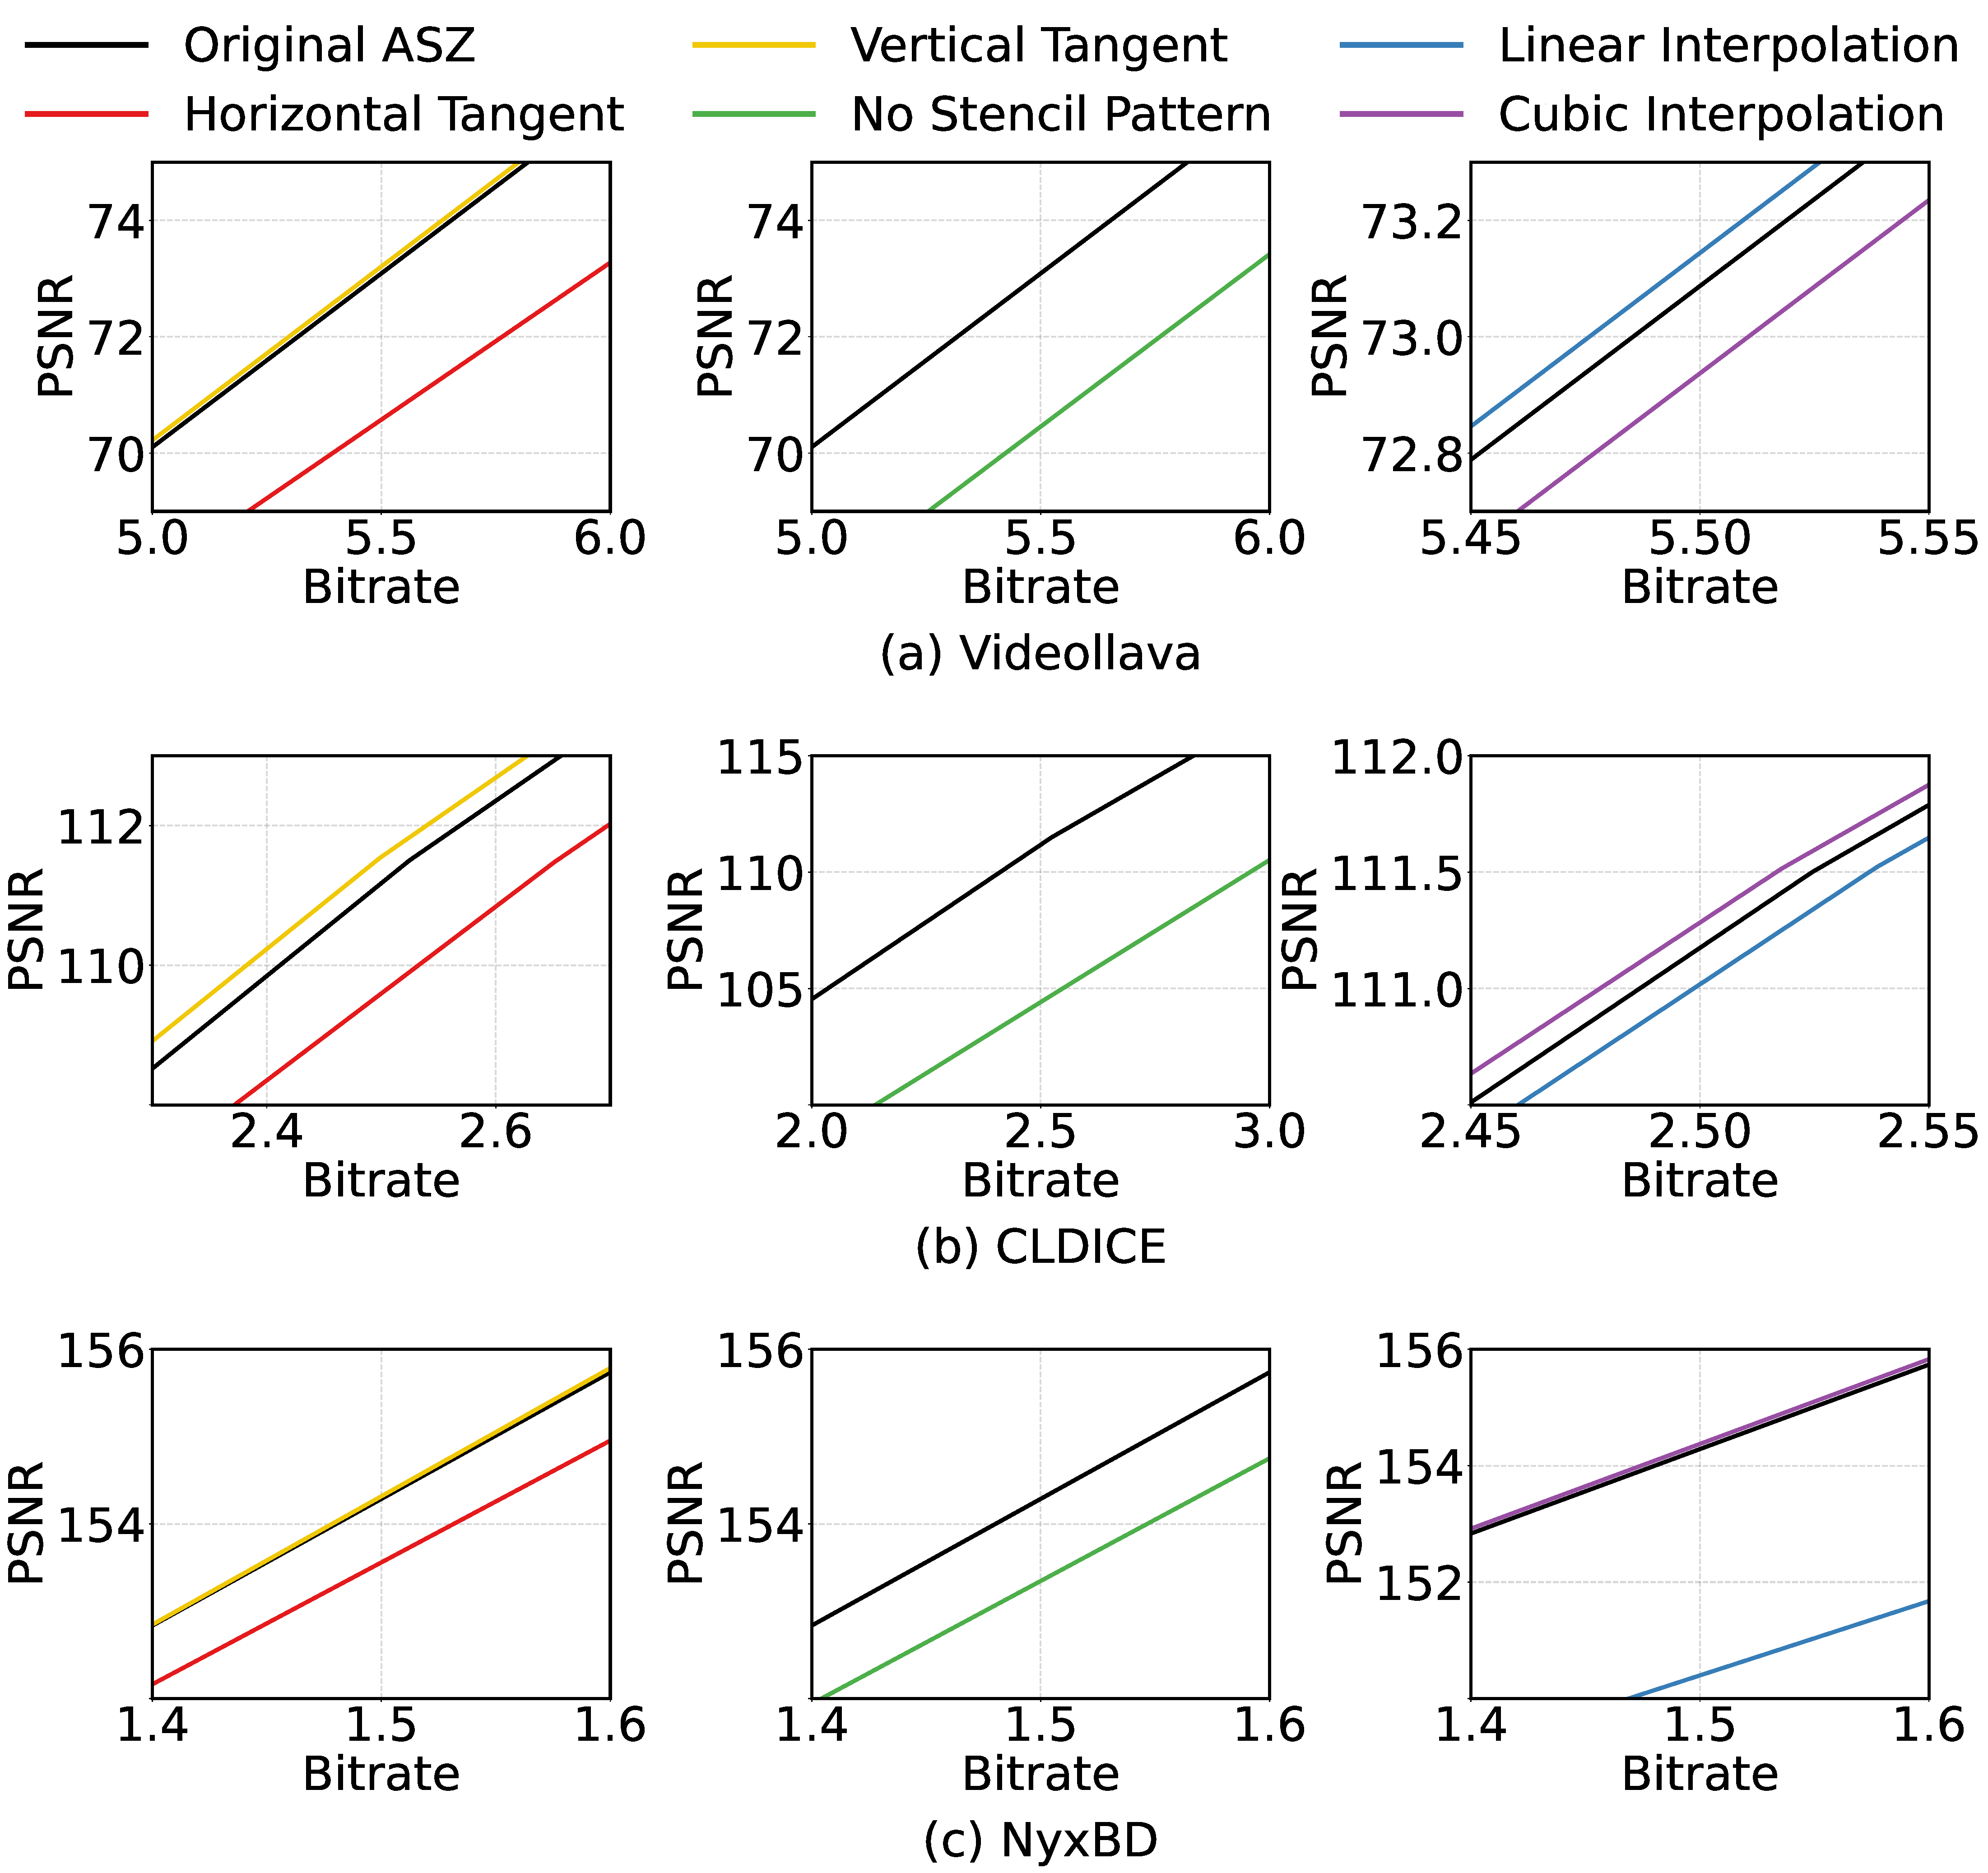
\includegraphics[width=1\linewidth]{figs/5/performance breakdown.pdf}
    \caption{Ablation study of major ASZ components.}
    \label{fig:performance breakdown}
\end{figure}

The first column of Figure~\ref{fig:performance breakdown} compares ASZ with two alternative configurations where the tangent direction is forced to be horizontal or vertical. We can observe that the rate-distortion curve of the vertical-tangent configuration is very close to that of ASZ. This is because, in most cases, the slope of the tangent estimated by ASZ ranges from approximately 5 to 5000 and therefore remains significantly larger than 1. From a geometric perspective, such steep tangent directions are much closer to the vertical case than to the horizontal case.

The second column compares ASZ-based stencil pattern selection with the default strategy that cyclically predicts along each dimension in order. The results show that allowing ASZ to adaptively select stencil patterns consistently achieves better rate-distortion performance.

The third column compares adaptive predictor coefficient selection in ASZ with fixed linear and cubic interpolation coefficients. In most cases, cubic interpolation outperforms linear interpolation, although there are also datasets where linear interpolation performs significantly better, such as Videollava. In several cases, using fixed coefficients can slightly outperform adaptive coefficient selection because coefficient storage overhead is eliminated. However, no single fixed predictor consistently performs best across all datasets and error-bound settings. ASZ provides a more robust and adaptive solution by dynamically selecting predictor coefficients according to the data characteristics and compression regime.

\subsection{Runtime Analysis}

In this section, we compare the runtime of ASZ with other baseline compressors and further analyze the runtime breakdown of ASZ. Specifically, we measure the time spent in the major stages of ASZ, including tangent estimation, stencil pattern selection, and compression. We additionally evaluate the runtime impact of disabling stencil pattern selection or adaptive coefficient tuning.

In Figure~\ref{fig:runtime}, we present the runtime of different compressors for compressing CLDICE with a relative error bound of $10^{-4}$ and NyxBD with a relative error bound of $10^{-6}$. We choose these two error bounds because they are located at the middle of the error-bound ranges shown in Figure~\ref{fig:rate-distortion}(c) and (d).

\begin{figure}
    \centering
    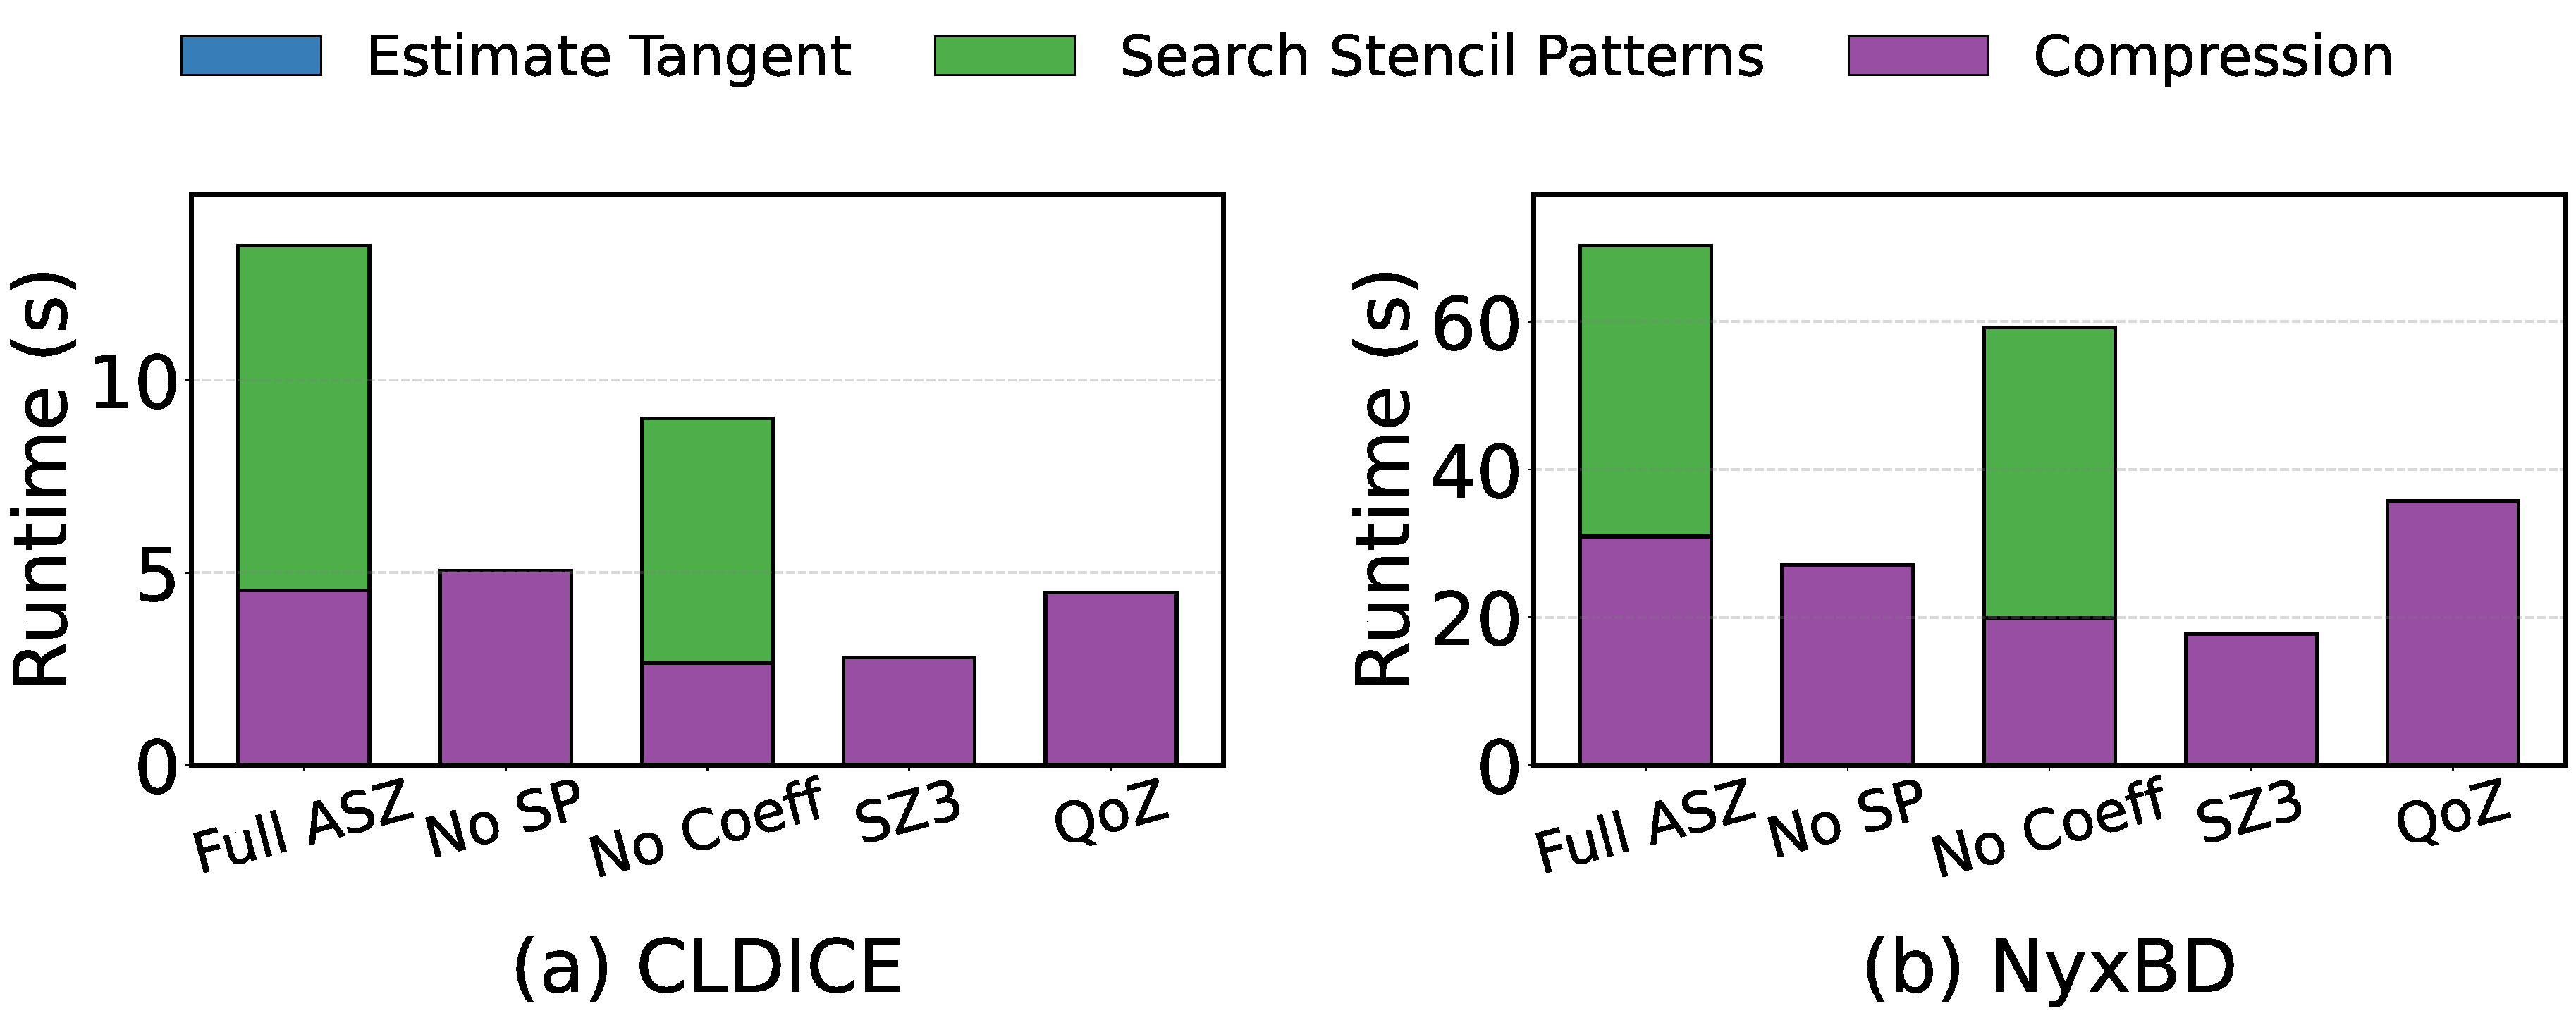
\includegraphics[width=1\linewidth]{figs/5/runtime.pdf}
    \caption{Runtime comparison and breakdown of ASZ and baseline compressors.}
    \label{fig:runtime}
\end{figure}

First, we can find that the runtime of tangent estimation is barely visible in the figure. This is because tangent estimation takes only about $5\times10^{-3}$ seconds, which is much smaller than the other stages and can be considered nearly free in practice.

Most of the runtime overhead of ASZ is spent on stencil pattern searching. However, stencil patterns can be selected offline in advance. In practice, such stencil patterns are often reusable across similar datasets, for example, datasets with the same shape generated by the same instrument or produced by the same simulation algorithm. The workflow involves selecting a representative dataset to estimate the tangent and determine the stencil patterns offline, and then, for each dataset to be compressed, ASZ only performs tangent estimation and compression using the preselected stencil patterns. Although tangent estimation still needs to be repeated for each dataset, its runtime overhead is negligible in practice. Excluding the overhead of stencil pattern search, the runtime of the compression stage in ASZ lies between that of SZ3 and QoZ.

Without stencil pattern selection, the runtime of the compression stage in ASZ may either increase or decrease. When suitable stencil patterns are not provided, the predictors in ASZ can produce quantized prediction errors with a more scattered distribution, which increases the runtime of the lossless compression stage in the SZ compression framework. Similar behavior has also been observed in SZ3 and QoZ. On the other hand, the default stencil patterns are designed to maximize contiguous memory access, which can reduce prediction overhead and improve runtime efficiency during prediction. These two effects compete with each other, and it is unclear which one will dominate in practice.

When stencil pattern selection is enabled while adaptive coefficient tuning is replaced with fixed third-order interpolation coefficients, the compression stage in ASZ can become even faster than that of SZ3.
\section{Discussion}\label{sec:discussion}
% The novelty remains limited, as the work appears to extend SZ/QoZ rather than introduce a fundamentally new compression approach.
% The tangent-based criterion is not clearly shown to be a major contributor.
% The broader applicability to ZFP, MGARD, SPERR, or AI-based compressors is not demonstrated.

% 改成“面向error-bounded compression的高效configuration exploration and optimization framework，ASZ是它在interpolation-based compression上的完整实例”
% 重新定义novelty
%   数学化“压缩配置搜索”问题
%   提出将可搜索的配置分为“压缩器设计者需要搜索的”、“用户对于一个数据集需要搜索的”、“用户对于特定数据文件可以online搜索的”
%   对于interpolation based compressor，哪些配置值得搜索？哪些配置不值得搜索？值得搜索的配置应该在哪里搜索？
%   ASZ 是实例，而不是全部贡献
% 一张design space表，表明SZ3、QoZ、ASZ的搜索空间的区别
% 更多的图来证明可以用h1-psnr替代bitrate-psnr，同时比较其他评价标准是否准确
% 遍历顺序也是一项需要搜索的配置
% 数学上分析cubic interpolation的系数理应非常普适，但也可能有其他系数在特定数据上更好
% 提出rate-distortion图像被严重拉伸，实际上的图像中的斜率不等于dPSNR/dBR，加入用户可以指定PSNR被拉伸的倍数的功能
% 提到data management，加上end to end测试
% 用一个表格挑一下rate-distortion中的几个点汇报数据
% introduction中加上asz相对于qoz的具体数值
% 提到参数跨eb的能力？

% 引用Automatic configuration tuning、Physical design optimization的相关文章，这个领域的主要目的是搜索诸如buffer size、thread count之类的配置，也会用到分层搜索

\section{Conclusion}\label{sec:conclusion}

In this paper, we propose ASZ, an adaptive prediction-based error-bounded lossy compressor that improves rate-distortion performance through systematic exploration of stencil patterns and predictor coefficients. By employing efficient predictor evaluation, ASZ is able to explore a substantially larger predictor space while still maintaining practical runtime overhead.

Experimental results on datasets from multiple domains demonstrate that ASZ consistently achieves better rate-distortion performance than state-of-the-art prediction-based compressors. Runtime analysis further shows that the additional overhead mainly comes from stencil pattern exploration, while tangent estimation and adaptive coefficient selection introduce relatively small costs. Moreover, the stencil-pattern exploration stage can potentially be amortized or reused across similar datasets, further improving the practicality of the framework. Overall, this work demonstrates that systematically enlarging the predictor search space is a promising direction for improving prediction-based error-bounded lossy compression.

There are several directions for future work. First, ASZ currently focuses on interpolation-based predictors with relatively simple tunable coefficients, while extending the framework to higher-order adaptive prediction functions may further improve compression performance. 
Second, improving the approximation of the actual bitrate may further improve the accuracy of the predictors. 
Finally, integrating ASZ with parallel and GPU-based compression frameworks is another promising direction for improving scalability and throughput.


column width = \the\columnwidth

\makeatletter
font size: \f@size pt
\makeatother

\begin{acks}
This research was supported by the U.S. Department of Energy, Office of Science, Advanced Scientific Computing Research (ASCR), under contract DE-AC02-06CH11357, and supported by the National Science Foundation under Grant OAC-2003709, OAC-2104023, OAC-2311875, OAC-2330367, OAC-2311756, and OAC-2313122. We acknowledge the computing resources provided on Bebop (operated by Laboratory Computing Resource Center at Argonne) and ACCESS Anvil machine operated by Purdue University.
\end{acks}

%\clearpage

\bibliographystyle{ACM-Reference-Format}
\bibliography{reference}

\end{document}
\endinput
